% =====================================================================
%  The Maps Behind LLMs: the decoder-only Transformer -- AMSOU Seminar (graduate students and faculty), Ohio University
%  Preamble follows the RLHF independent-study template
%  ("From the Reward Model to DPO"); TikZ libraries and the operator
%  macros for the board notation (Attn.B, FFN.B, ...) are added.
%  Notation follows the board formulas in First-transformer.ipynb.
% =====================================================================
\documentclass[aspectratio=169,11pt]{beamer}
\usepackage[utf8]{inputenc}
\usepackage{amsmath,amssymb,amscd,mathtools}
\usepackage{booktabs,tabularx,array}
\usepackage{tikz}
\usetikzlibrary{arrows.meta,positioning,calc,decorations.pathreplacing,fit,backgrounds}
\usepackage[most]{tcolorbox}
\usefonttheme{serif}
\usetheme{default}
\setbeamertemplate{navigation symbols}{}
% Ohio University palette (ohio.edu/brand/visual-identity/colors)
\definecolor{acc}{HTML}{00694E}   % Cutler Green (dominant)
\definecolor{tea}{HTML}{024230}   % Under the Elms
\definecolor{gld}{HTML}{AA8A00}   % Marigold (accent)
\definecolor{gry}{HTML}{756E65}   % Putnam
\definecolor{syc}{HTML}{E7ECC3}   % Sycamore
\definecolor{tri}{HTML}{F9F7ED}   % Trillium
\definecolor{rust}{HTML}{FA4616}  % Rust (accent)
\setbeamercolor{structure}{fg=acc}
\setbeamercolor{frametitle}{fg=black}
\setbeamercolor{frametitle bar}{fg=white,bg=acc}
\setbeamertemplate{frametitle}{\nointerlineskip\begin{beamercolorbox}[wd=\paperwidth,ht=3.1ex,dp=1.2ex,leftskip=1.1em,rightskip=1.0em]{frametitle bar}\usebeamerfont{frametitle}\insertframetitle\hfill{\normalfont\tiny\crumbbox}\end{beamercolorbox}\par\vskip0.6ex}
% ---- funnel breadcrumbs (shown at the right of the title bar)
\newcommand{\crumbbox}{}
\newcommand{\ci}[2]{\ifnum#1=\crumbk\relax{\setlength{\fboxsep}{1.2pt}\colorbox{white}{\color{acc}\bfseries #2}}\else{\color{white!70!acc}#2}\fi}
\newcommand{\crar}{{\color{white!70!acc}$\,\rightarrow\,$}}
\newcommand{\crumbsA}[1]{\gdef\crumbbox{\def\crumbk{#1}\ci{1}{$\AttnB$}\crar\ci{2}{$\MHA_M$}\crar\ci{3}{$\Attn^M_r$}\crar\ci{4}{$S$, softmax}\crar\ci{5}{mask $M$}\crar\ci{6}{$\oplus$, $\LN$}}}
\newcommand{\crumbsF}[1]{\gdef\crumbbox{\def\crumbk{#1}\ci{1}{$\FFNB$}\crar\ci{2}{row-wise}\crar\ci{3}{$\FFN(u)$}}}
\newcommand{\crumbsoff}{\gdef\crumbbox{}}
\setbeamerfont{frametitle}{size=\large,series=\bfseries}
\setbeamertemplate{footline}{\leavevmode{\color{acc}\rule{\paperwidth}{0.6pt}}\par\vskip0.3ex\hspace*{1em}{\tiny\color{gry}\insertsection}\hfill{\tiny\color{acc}\insertframenumber/\inserttotalframenumber}\hspace*{1em}\vskip0.9ex}
\setbeamertemplate{itemize items}[circle]
\setbeamerfont{itemize/enumerate body}{size=\small}
\newcommand{\E}{\mathbb{E}}\newcommand{\R}{\mathbb{R}}\renewcommand{\P}{\mathbb{P}}\newcommand{\N}{\mathbb{N}}
\newcommand{\KL}{\operatorname{KL}}
\newcommand{\argmax}{\operatorname*{arg\,max}}\newcommand{\argmin}{\operatorname*{arg\,min}}
\tcbset{enhanced,boxrule=0pt,leftrule=2.2pt,arc=1pt,top=3pt,bottom=3pt,left=6pt,right=5pt,before skip=4pt,after skip=4pt,fontupper=\normalsize,halign=flush left}
\newtcolorbox{bxthm}{colback=gld!10,colframe=gld}   % theorem / proposition / check
\newtcolorbox{bxdef}{colback=acc!8,colframe=acc}    % definition / boxed objective
\newtcolorbox{bxrem}{colback=syc!55,colframe=tea}  % remark / interpretation
\newtcolorbox{bxalg}{colback=tri,colframe=gry}      % algorithm
\newcolumntype{Y}{>{\raggedright\arraybackslash}X}

% ---- board notation ---------------------------------------------------
\newcommand{\Attn}{\operatorname{Attn}}
\newcommand{\AttnB}{\operatorname{Attn{.}B}}
\newcommand{\FFNB}{\operatorname{FFN{.}B}}
\newcommand{\CAttn}{\operatorname{CAttn}}
\newcommand{\CAttnB}{\operatorname{CAttn{.}B}}
\newcommand{\cfix}{\vspace{-\baselineskip}}% column that starts with a box
\newcommand{\FFN}{\operatorname{FFN}}
\newcommand{\MHA}{\operatorname{MHA}}
\newcommand{\LN}{\operatorname{LN}}
\newcommand{\DL}{\operatorname{DL}}
\newcommand{\EL}{\operatorname{EL}}
\newcommand{\relu}{\operatorname{relu}}
\newcommand{\softmax}{\operatorname{softmax}}
\newcommand{\Concat}{\operatorname{Concat}}
\newcommand{\Emb}{\operatorname{Emb}}
\newcommand{\Vc}{\mathcal V}
\newcommand{\one}{\mathbf 1}
\newcommand{\dff}{d_{\mathrm{ff}}}
\newcommand{\Wv}{W_{\mathrm{vocab}}}
% overlay-aware TikZ visibility
\tikzset{invisible/.style={opacity=0,text opacity=0},
  visible on/.style={alt={#1{}{invisible}}},
  alt/.code args={<#1>#2#3}{\alt<#1>{\pgfkeysalso{#2}}{\pgfkeysalso{#3}}}}
\tikzset{blk/.style={draw=#1,thick,fill=#1!8,rounded corners=1.5pt,inner sep=1pt},
  blkA/.style={blk=#1,minimum width=2.5cm,minimum height=0.42cm},
  blkB/.style={blk=#1,minimum width=2.2cm,minimum height=0.55cm},
  big/.style={draw=#1,thick,fill=#1!10,rounded corners=3pt,minimum width=3.0cm,minimum height=0.95cm,align=center},
  hb/.style={draw=#1,thick,fill=#1!8,rounded corners=2pt,minimum width=3.3cm,minimum height=0.85cm,align=center}}

\title{The decoder-only Transformer}
\subtitle{The Maps Behind LLM}
\author{}
\date{}

\begin{document}

% ---------- Title frame -----------------------------------------------
{\setbeamercolor{background canvas}{bg=acc}
\begin{frame}[plain]
\begin{tikzpicture}[remember picture,overlay]
% bottom band with a marigold rule
\fill[tea] (current page.south west) rectangle ([yshift=1.3cm]current page.south east);
\fill[gld] ([yshift=1.3cm]current page.south west) rectangle ([yshift=1.36cm]current page.south east);
% causal attention pattern (lower triangle) as a motif
\begin{scope}[shift={($(current page.north east)+(-5.75,-1.5)$)}]
\def\c{0.52}
\foreach \i in {1,...,8}{\foreach \j in {1,...,8}{
  \ifnum\j>\i
    \draw[white,opacity=0.16,line width=0.4pt] ({\c*(\j-1)+0.03},{-\c*\i+0.03}) rectangle ({\c*\j-0.03},{-\c*(\i-1)-0.03});
  \else
    \pgfmathsetmacro{\op}{0.14+0.075*mod(\i*7+\j*4,9)}
    \fill[white,opacity=\op] ({\c*(\j-1)+0.03},{-\c*\i+0.03}) rectangle ({\c*\j-0.03},{-\c*(\i-1)-0.03});
  \fi
}}
\node[anchor=north,text=white,opacity=0.85,font=\footnotesize] at ({4*\c},{-8*\c-0.12}) {$A=\softmax_{\rm row}\!\big(QK^\top/\sqrt{d_k}+M\big)$};
\end{scope}
% title block
\fill[white] ($(current page.south west)+(0.95,2.95)$) rectangle ($(current page.south west)+(1.03,6.95)$);
\node[anchor=north west,text=white,align=left,inner sep=0pt,font=\huge\bfseries] at ($(current page.south west)+(1.35,6.95)$)
  {The decoder-only\\[3pt]Transformer};
\node[anchor=north west,text=syc,inner sep=0pt] at ($(current page.south west)+(1.35,4.85)$)
  {\Large The Maps Behind LLM};
\draw[white!70!acc,line width=0.6pt] ($(current page.south west)+(1.35,3.95)$) -- ++(4.6,0);
\node[anchor=north west,text=white!88!acc,inner sep=0pt] at ($(current page.south west)+(1.35,3.6)$)
  {\small AMSOU Seminar \,\textperiodcentered\, Department of Mathematics};
% token strip in the band
\begin{scope}[shift={($(current page.south west)+(1.35,0.65)$)},
  tk/.style={draw=white,rounded corners=2pt,text=white,font=\scriptsize\itshape,inner sep=3pt,minimum height=0.45cm}]
\node[tk,anchor=west] (t1) at (0,0) {The};
\node[tk,right=0.18cm of t1] (t2) {model};
\node[tk,right=0.18cm of t2] (t3) {reads};
\node[tk,right=0.18cm of t3] (t4) {one};
\node[tk,right=0.18cm of t4,draw=gld,fill=gld,text=white,font=\scriptsize\bfseries] (t5) {?};
\node[right=0.45cm of t5,text=white,font=\small] {$p_i=\pi_\theta(\,\cdot\mid y_{\le i})$};
\end{scope}
\end{tikzpicture}
\end{frame}}

% ---------- What an LM computes ---------------------------------------
\begin{frame}[t]{What a language model computes}
\begin{columns}[T]
\begin{column}{0.55\textwidth}
\cfix
\begin{center}
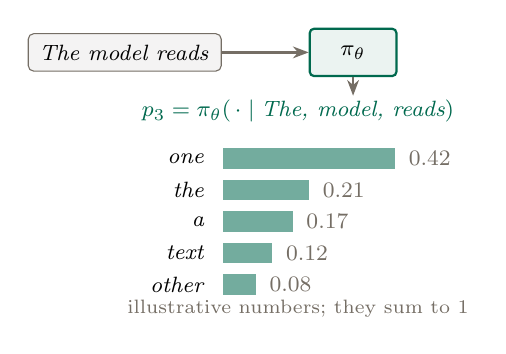
\begin{tikzpicture}[every node/.style={font=\footnotesize},>={Stealth[length=2mm]}]
\node[draw=gry,rounded corners=2pt,fill=gry!8,inner sep=4pt] (pre) at (0,3.2) {\textit{The model reads}};
\node[blk=acc,minimum width=1.1cm,minimum height=0.6cm] (pi) at (2.9,3.2) {$\pi_\theta$};
\draw[->,gry,thick] (pre) -- (pi);
\node[text=acc] at (2.2,2.45) {$p_3=\pi_\theta(\,\cdot\mid\textit{The, model, reads})$};
\foreach \t/\p/\k in {one/0.42/0,the/0.21/1,a/0.17/2,text/0.12/3,{other}/0.08/4}{
  \node[anchor=east] at (1.15,{1.85-0.4*\k}) {\textit{\t}};
  \fill[acc!55] (1.25,{1.85-0.4*\k-0.13}) rectangle ({1.25+5.2*\p},{1.85-0.4*\k+0.13});
  \node[anchor=west,text=gry] at ({1.3+5.2*\p},{1.85-0.4*\k}) {\p};
}
\draw[->,gry,thick] (pi) -- (2.9,2.65);
\node[text=gry,font=\scriptsize] at (2.2,-0.05) {illustrative numbers; they sum to $1$};
\end{tikzpicture}
\end{center}
\begin{bxrem}
\textbf{Generation.} $y_{n+1}\sim p_n$, append, repeat.
\end{bxrem}
\end{column}
\begin{column}{0.42\textwidth}
\cfix
\begin{center}
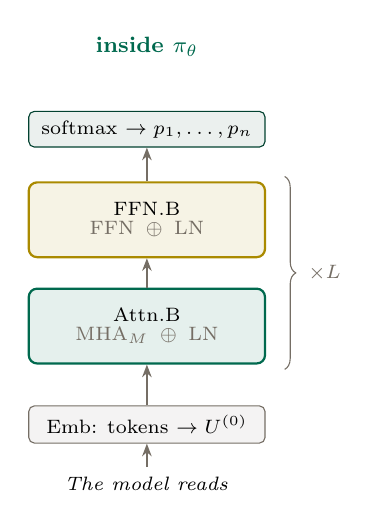
\begin{tikzpicture}[every node/.style={font=\scriptsize},>={Stealth[length=1.6mm]}]
\node[text=acc,font=\footnotesize\bfseries] at (0,5.55) {inside $\pi_\theta$};
\node (in) at (0,0) {\textit{The model reads}};
\node[draw=gry,rounded corners=2pt,fill=gry!8,minimum width=3.0cm,minimum height=0.45cm] (emb) at (0,0.75) {$\Emb$: tokens $\to U^{(0)}$};
\node[big=acc] (ab) at (0,2.0) {\textbf{$\AttnB$}\\[-1pt]{\color{gry}$\MHA_M\ \oplus\ \LN$}};
\node[big=gld] (fb) at (0,3.35) {\textbf{$\FFNB$}\\[-1pt]{\color{gry}$\FFN\ \oplus\ \LN$}};
\node[draw=tea,rounded corners=2pt,fill=tea!8,minimum width=3.0cm,minimum height=0.45cm] (sm) at (0,4.5) {softmax $\to p_1,\dots,p_n$};
\draw[->,gry,thick] (in)--(emb); \draw[->,gry,thick] (emb)--(ab); \draw[->,gry,thick] (ab)--(fb); \draw[->,gry,thick] (fb)--(sm);
\draw[decorate,decoration={brace,amplitude=4pt},gry] (1.75,3.9) -- node[right=5pt]{$\times L$} (1.75,1.45);
\end{tikzpicture}
\end{center}
\end{column}
\end{columns}
\end{frame}

% ---------- Road map --------------------------------------------------
\begin{frame}{The road map}
\begin{center}
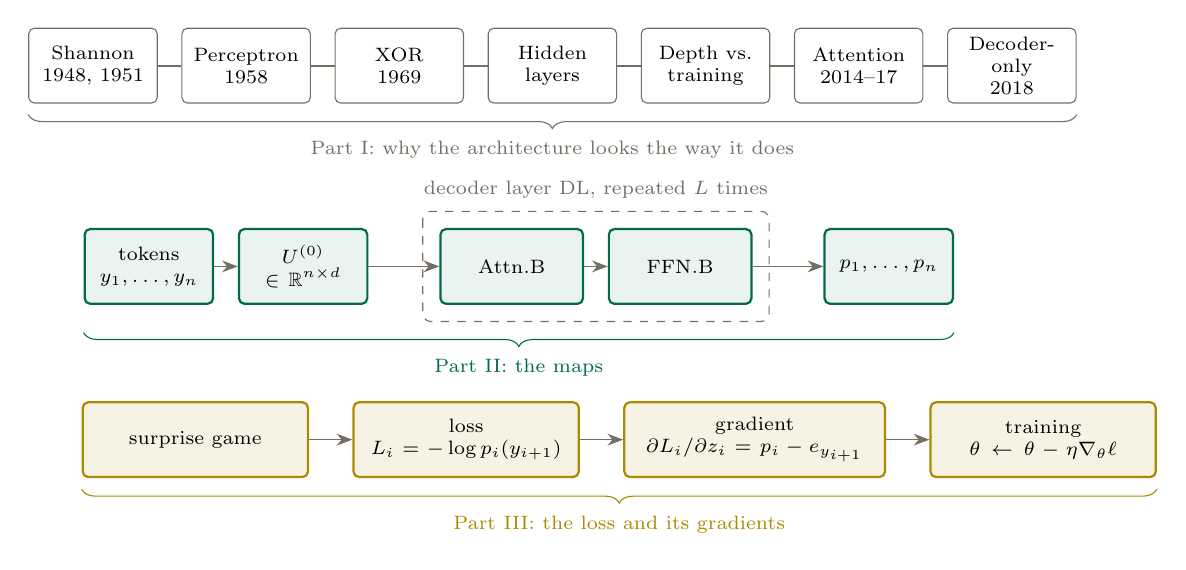
\begin{tikzpicture}[node distance=0.3cm,
  every node/.style={font=\scriptsize},
  box/.style={draw=gry,rounded corners=2pt,inner sep=3pt,align=center,minimum height=0.95cm,text width=1.42cm},
  hot/.style={box,draw=acc,fill=acc!8,thick},
  ar/.style={-{Stealth[length=2mm]},gry}]
\node[box] (a) {Shannon\\1948, 1951};
\node[box,right=of a] (b) {Perceptron\\1958};
\node[box,right=of b] (c) {XOR\\1969};
\node[box,right=of c] (d) {Hidden\\layers};
\node[box,right=of d] (e) {Depth vs.\\training};
\node[box,right=of e] (f) {Attention\\2014--17};
\node[box,right=of f] (g) {Decoder-only\\2018};
\foreach \u/\v in {a/b,b/c,c/d,d/e,e/f,f/g} \draw[gry,thick] (\u) -- (\v);
\draw[decorate,decoration={brace,mirror,amplitude=5pt},gry]
  ([yshift=-4pt]a.south west) -- node[below=6pt]{Part I: why the architecture looks the way it does} ([yshift=-4pt]g.south east);
\begin{scope}[yshift=-2.55cm]
\node[hot] (t) at (0.71,0) {tokens\\$y_1,\dots,y_n$};
\node[hot,right=of t] (u) {$U^{(0)}$\\$\in\R^{n\times d}$};
\node[hot,right=0.9cm of u,text width=1.6cm] (ca) {$\AttnB$};
\node[hot,right=of ca,text width=1.6cm] (ff) {$\FFNB$};
\node[hot,right=0.9cm of ff] (p) {$p_1,\dots,p_n$};
\draw[ar] (t)--(u); \draw[ar] (u)--(ca); \draw[ar] (ca)--(ff); \draw[ar] (ff)--(p);
\draw[gry,dashed,rounded corners=3pt] ([xshift=-6pt,yshift=6pt]ca.north west) rectangle ([xshift=6pt,yshift=-6pt]ff.south east);
\node[text=gry,anchor=south] at ($(ca.north east)!0.5!(ff.north west)+(0,0.25)$) {decoder layer $\DL$, repeated $L$ times};
\draw[decorate,decoration={brace,mirror,amplitude=5pt},acc]
  ([yshift=-10pt]t.south west) -- node[below=6pt,text=acc]{Part II: the maps} ([yshift=-10pt]p.south east);
\end{scope}
\begin{scope}[yshift=-4.75cm,hot3/.style={box,draw=gld,fill=gld!10,thick,text width=2.65cm}]
\node[hot3] (g1) at (1.3,0) {surprise game};
\node[hot3,right=0.55cm of g1] (g2) {loss\\$L_i=-\log p_i(y_{i+1})$};
\node[hot3,right=0.55cm of g2,text width=3.1cm] (g3) {gradient\\$\partial L_i/\partial z_i=p_i-e_{y_{i+1}}$};
\node[hot3,right=0.55cm of g3] (g4) {training\\$\theta\leftarrow\theta-\eta\nabla_\theta\ell$};
\draw[ar] (g1)--(g2); \draw[ar] (g2)--(g3); \draw[ar] (g3)--(g4);
\draw[decorate,decoration={brace,mirror,amplitude=5pt},gld]
  ([yshift=-4pt]g1.south west) -- node[below=6pt,text=gld]{Part III: the loss and its gradients} ([yshift=-4pt]g4.south east);
\end{scope}
\end{tikzpicture}
\end{center}
\end{frame}

%==================================================
\section{History}

% ---------- Timeline --------------------------------------------------
\begin{frame}{A short history}
\begin{center}
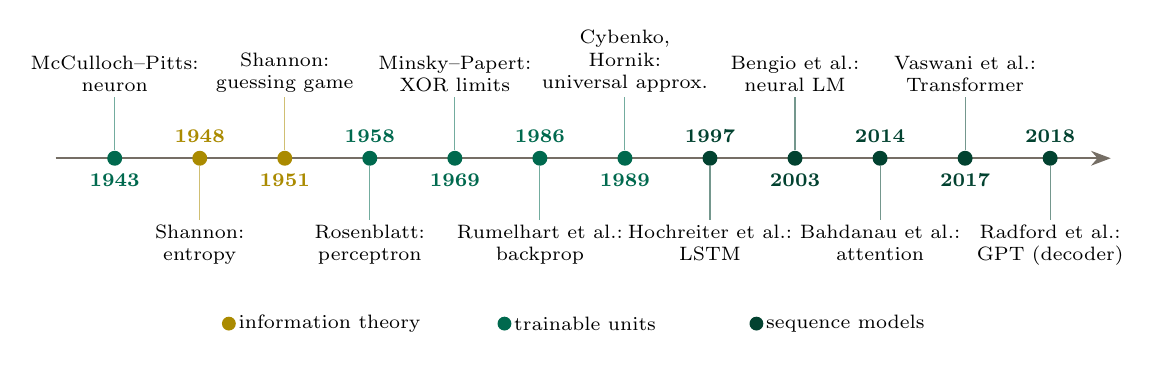
\begin{tikzpicture}[every node/.style={font=\scriptsize}]
\draw[gry,thick,-{Stealth[length=2.5mm]}] (-0.2,0) -- (13.2,0);
\foreach \k/\yr/\txt/\col in {
 0/1943/{McCulloch--Pitts:\\neuron}/acc,
 1/1948/{Shannon:\\entropy}/gld,
 2/1951/{Shannon:\\guessing game}/gld,
 3/1958/{Rosenblatt:\\perceptron}/acc,
 4/1969/{Minsky--Papert:\\XOR limits}/acc,
 5/1986/{Rumelhart et al.:\\backprop}/acc,
 6/1989/{Cybenko, Hornik:\\universal approx.}/acc,
 7/1997/{Hochreiter et al.:\\LSTM}/tea,
 8/2003/{Bengio et al.:\\neural LM}/tea,
 9/2014/{Bahdanau et al.:\\attention}/tea,
 10/2017/{Vaswani et al.:\\Transformer}/tea,
 11/2018/{Radford et al.:\\GPT (decoder)}/tea}{
  \pgfmathsetmacro{\x}{0.55+1.08*\k}
  \pgfmathtruncatemacro{\up}{mod(\k,2)}
  \fill[\col] (\x,0) circle (2.7pt);
  \ifnum\up=0
    \draw[\col!55] (\x,0.1) -- (\x,0.78);
    \node[above,align=center,text width=2.14cm,inner sep=1pt] at (\x,0.8) {\txt};
    \node[below,text=\col,font=\scriptsize\bfseries] at (\x,-0.08) {\yr};
  \else
    \draw[\col!55] (\x,-0.1) -- (\x,-0.78);
    \node[below,align=center,text width=2.14cm,inner sep=1pt] at (\x,-0.8) {\txt};
    \node[above,text=\col,font=\scriptsize\bfseries] at (\x,0.08) {\yr};
  \fi
}
\fill[gld] (2.0,-2.1) circle (2.5pt) node[right,text=black]{information theory};
\fill[acc] (5.5,-2.1) circle (2.5pt) node[right,text=black]{trainable units};
\fill[tea] (8.7,-2.1) circle (2.5pt) node[right,text=black]{sequence models};
\end{tikzpicture}
\end{center}
\begin{bxrem}
Three threads meet in 2017: Shannon's \emph{next-symbol} objective, Rosenblatt's \emph{trainable units}, and \emph{attention}.
\end{bxrem}
\end{frame}

% ---------- Shannon ---------------------------------------------------
\begin{frame}[t]{Shannon (1948, 1951): language as a stochastic process}
\begin{bxdef}
\textbf{Entropy rate.} $(Y_t)_{t\ge1}$ stationary on a finite alphabet $\Vc$:
\[
H_\infty=\lim_{n\to\infty}H(Y_n\mid Y_1,\dots,Y_{n-1}),\qquad
H(Y_n\mid Y_{<n})=-\E\log_2\P(Y_n\mid Y_{<n}).
\]
\end{bxdef}
\begin{columns}[T]
\begin{column}{0.45\textwidth}
\vspace{0.1cm}
\textbf{1948: $k$-gram} \ {\small($Y_t$ letters, $W_t$ words)}
{\small\begin{align*}
\P(Y_n\mid Y_{<n})&\approx\P(Y_n\mid Y_{n-k},\dots,Y_{n-1})\\
\P(W_n\mid W_{<n})&\approx\P(W_n\mid W_{n-k},\dots,W_{n-1})
\end{align*}}
\textbf{1951: English}\\[2pt] $0.6\lesssim H_\infty\lesssim1.3$ bits/letter
\end{column}
\begin{column}{0.52\textwidth}
\begin{center}
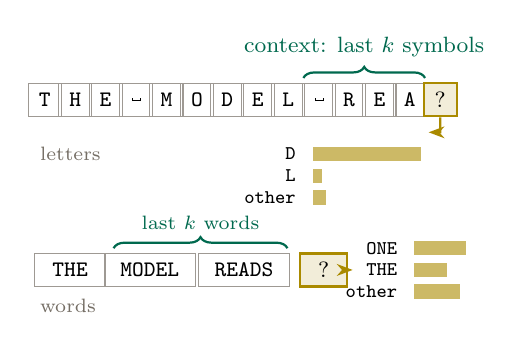
\begin{tikzpicture}[scale=0.92,every node/.style={font=\footnotesize},>={Stealth[length=2mm]}]
\def\w{0.42}
\foreach \ch [count=\k from 0] in {T,H,E,{\textvisiblespace},M,O,D,E,L,{\textvisiblespace},R,E,A}{
  \node[draw=gry!70,minimum size=\w cm,inner sep=0pt,font=\ttfamily\footnotesize] at ({\w*\k},0) {\ch};
}
\node[draw=gld,thick,fill=gld!15,minimum size=\w cm,inner sep=0pt] (q) at ({\w*13},0) {?};
\draw[decorate,decoration={brace,amplitude=4pt},acc,thick] ({\w*8.5},0.3) -- node[above=4pt,text=acc]{context: last $k$ symbols} ({\w*12.5},0.3);
\foreach \t/\p/\k in {D/0.83/0,L/0.07/1,other/0.10/2}{
  \node[anchor=east,font=\ttfamily\scriptsize] at (3.6,{-0.75-0.3*\k}) {\t};
  \fill[gld!60] (3.7,{-0.75-0.3*\k-0.1}) rectangle ({3.7+1.8*\p},{-0.75-0.3*\k+0.1});
}
\draw[->,gld,thick] (q.south) -- ({\w*13},-0.45) -- (5.3,-0.45);
\node[anchor=west,text=gry,font=\scriptsize] at (-0.2,-0.75) {letters};
% word strip
\begin{scope}[yshift=-2.35cm]
\foreach \wrd/\x/\wwd in {THE/0.35/0.9,MODEL/1.45/1.15,READS/2.75/1.15}{
  \node[draw=gry!70,minimum height=\w cm,minimum width=\wwd cm,inner sep=1pt,font=\ttfamily\footnotesize] at (\x,0) {\wrd};}
\node[draw=gld,thick,fill=gld!15,minimum height=\w cm,minimum width=0.6cm,inner sep=0pt] (qw) at (3.85,0) {?};
\draw[decorate,decoration={brace,amplitude=4pt},acc,thick] (0.95,0.3) -- node[above=3pt,text=acc,font=\scriptsize]{last $k$ words} (3.35,0.3);
\foreach \t/\p/\k in {ONE/0.40/0,THE/0.25/1,other/0.35/2}{
  \node[anchor=east,font=\ttfamily\scriptsize] at (5.0,{0.3-0.3*\k}) {\t};
  \fill[gld!60] (5.1,{0.3-0.3*\k-0.1}) rectangle ({5.1+1.8*\p},{0.3-0.3*\k+0.1});
}
\draw[->,gld,thick] (qw.east) -- (4.25,0);
\node[anchor=west,text=gry,font=\scriptsize] at (-0.2,-0.5) {words};
\end{scope}
\end{tikzpicture}
\end{center}
\end{column}
\end{columns}
\begin{bxrem}
\textbf{LLM loss} (cross-entropy):\quad $L_i=-\log p_i(y_{i+1})$.
\end{bxrem}
\end{frame}

% ---------- Perceptron ------------------------------------------------
\begin{frame}[t]{Rosenblatt (1958): the perceptron}
\begin{columns}[T]
\begin{column}{0.5\textwidth}
\cfix
\begin{center}
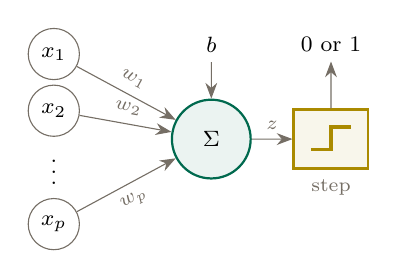
\begin{tikzpicture}[scale=0.8,every node/.style={font=\footnotesize},>={Stealth[length=2mm]}]
\foreach \i/\lab/\yy in {1/x_1/0,2/x_2/-0.9,4/x_p/-2.7}
  \node[circle,draw=gry,minimum size=6.5mm,inner sep=0pt] (x\i) at (0,\yy) {$\lab$};
\node at (0,-1.75) {$\vdots$};
\node[circle,draw=acc,thick,fill=acc!8,minimum size=10mm] (s) at (2.5,-1.35) {$\Sigma$};
\draw[->,gry] (x1) -- node[above,sloped,font=\scriptsize]{$w_1$} (s);
\draw[->,gry] (x2) -- node[above,sloped,font=\scriptsize]{$w_2$} (s);
\draw[->,gry] (x4) -- node[below,sloped,font=\scriptsize]{$w_p$} (s);
\node (bb) at (2.5,0.15) {$b$};
\draw[->,gry] (bb) -- (s);
\node[draw=gld,thick,fill=gld!8,minimum width=0.95cm,minimum height=0.75cm] (st) at (4.4,-1.35) {};
\draw[gld,very thick] ($(st.center)+(-0.32,-0.17)$) -- ($(st.center)+(0,-0.17)$) -- ($(st.center)+(0,0.19)$) -- ($(st.center)+(0.32,0.19)$);
\draw[->,gry] (s) -- node[above,font=\scriptsize]{$z$} (st);
\node[below,font=\scriptsize,text=gry] at (st.south) {step};
\node (out) at (4.4,0.15) {$0$ or $1$};
\draw[->,gry] (st) -- (out);
\end{tikzpicture}
\end{center}
\begin{bxdef}
\small\textbf{Trained:} $(w,b)\in\R^p\times\R$.
\begin{gather*}
f_{w,b}:\R^p\to\{0,1\}\\
f_{w,b}(x)=\one\{w^\top x+b>0\}
\end{gather*}
\end{bxdef}
\end{column}
\begin{column}{0.47\textwidth}
\cfix
\begin{center}
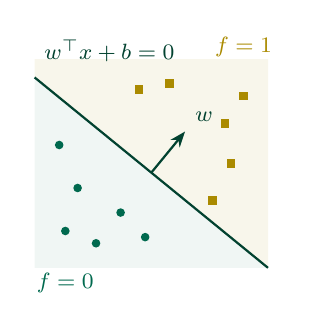
\begin{tikzpicture}[scale=0.78,every node/.style={font=\footnotesize},>={Stealth[length=2mm]}]
\fill[acc!6] (-0.2,-0.2) -- (3.6,-0.2) -- (-0.2,2.9) -- cycle;
\fill[gld!8] (3.6,-0.2) -- (3.6,3.2) -- (-0.2,3.2) -- (-0.2,2.9) -- cycle;
\draw[tea,thick] (-0.2,2.9) -- (3.6,-0.2);
\draw[->,tea,thick] (1.7,1.35) -- (2.25,2.02) node[above right]{$w$};
\foreach \px/\py in {0.3/0.4,0.8/0.2,0.5/1.1,1.2/0.7,0.2/1.8,1.6/0.3} \fill[acc] (\px,\py) circle (0.07);
\foreach \px/\py in {2.9/2.15,3.0/1.5,2.0/2.8,3.2/2.6,2.7/0.9,1.5/2.7} \fill[gld] ({\px-0.07},{\py-0.07}) rectangle ({\px+0.07},{\py+0.07});
\node[text=acc] at (0.3,-0.45) {$f=0$};
\node[text=gld] at (3.2,3.4) {$f=1$};
\node[text=tea,anchor=south west] at (-0.2,3.0) {$w^\top x+b=0$};
\end{tikzpicture}
\end{center}
\begin{bxalg}
\small\textbf{Learning rule.} Data $(x,t)$, $t\in\{0,1\}$, step $\eta>0$:
\[
(w,b)\leftarrow(w,b)+\eta\,\big(t-f_{w,b}(x)\big)\,(x,1)
\]
\end{bxalg}
\end{column}
\end{columns}
\end{frame}

% ---------- XOR -------------------------------------------------------
\begin{frame}[t]{Minsky--Papert (1969): XOR defeats one line}
\begin{columns}[T]
\begin{column}{0.4\textwidth}
\vspace{0.4cm}
\begin{center}
{\small
\begin{tabular}{cc|c}
\toprule
$x_1$ & $x_2$ & $x_1\oplus x_2$\\
\midrule
0 & 0 & {\color{acc}0}\\
1 & 0 & {\color{gld}1}\\
0 & 1 & {\color{gld}1}\\
1 & 1 & {\color{acc}0}\\
\bottomrule
\end{tabular}}
\end{center}
\vspace{0.5em}

\end{column}
\begin{column}{0.56\textwidth}
\cfix
\begin{center}
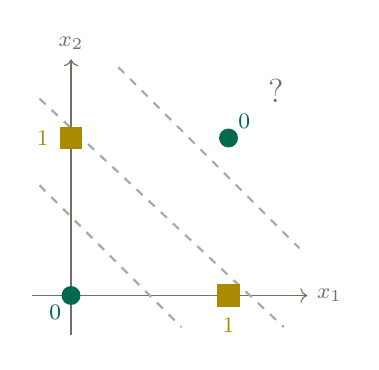
\begin{tikzpicture}[scale=2.0,every node/.style={font=\footnotesize}]
\draw[->,gry] (-0.25,0) -- (1.5,0) node[right]{$x_1$};
\draw[->,gry] (0,-0.25) -- (0,1.5) node[above]{$x_2$};
\draw[gry!60,dashed,thick] (-0.2,0.7) -- (0.7,-0.2);
\draw[gry!60,dashed,thick] (0.3,1.45) -- (1.45,0.3);
\draw[gry!60,dashed,thick] (-0.2,1.25) -- (1.35,-0.2);
\fill[acc] (0,0) circle (0.06);
\node[below left,text=acc] at (0,0) {$0$};
\fill[acc] (1,1) circle (0.06);
\node[above right,text=acc] at (1,1) {$0$};
\fill[gld] (0.93,-0.07) rectangle (1.07,0.07);
\node[below,text=gld] at (1,-0.08) {$1$};
\fill[gld] (-0.07,0.93) rectangle (0.07,1.07);
\node[left,text=gld] at (-0.08,1) {$1$};
\node[text=gry,font=\large] at (1.3,1.3) {?};
\end{tikzpicture}
\end{center}
\end{column}
\end{columns}
\begin{bxthm}
\textbf{Proposition.} There is no $(w,b)\in\R^2\times\R$ with $f_{w,b}(x)=x_1\oplus x_2$ for all $x\in\{0,1\}^2$.
\end{bxthm}
\end{frame}

% ---------- MLP solves XOR -------------------------------------------
\begin{frame}[t]{A hidden layer solves XOR}
\begin{columns}[T]
\begin{column}{0.45\textwidth}
\cfix
\begin{center}
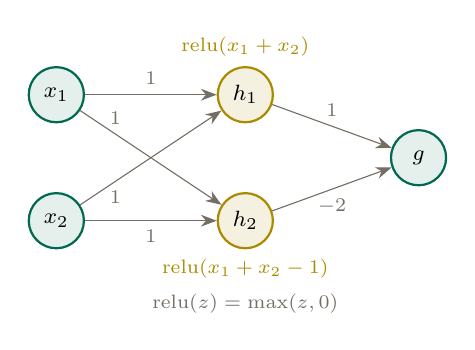
\begin{tikzpicture}[every node/.style={font=\footnotesize},>={Stealth[length=2mm]},
  ni/.style={circle,draw=acc,thick,fill=acc!10,minimum size=7mm,inner sep=0pt},
  nh/.style={circle,draw=gld,thick,fill=gld!12,minimum size=7mm,inner sep=0pt}]
\node[ni] (x1) at (0,1.6) {$x_1$};
\node[ni] (x2) at (0,0) {$x_2$};
\node[nh] (h1) at (2.4,1.6) {$h_1$};
\node[nh] (h2) at (2.4,0) {$h_2$};
\node[ni] (g) at (4.6,0.8) {$g$};
\draw[->,gry] (x1) -- node[above,font=\scriptsize]{$1$} (h1);
\draw[->,gry] (x1) -- node[pos=0.25,above,font=\scriptsize]{$1$} (h2);
\draw[->,gry] (x2) -- node[pos=0.25,below,font=\scriptsize]{$1$} (h1);
\draw[->,gry] (x2) -- node[below,font=\scriptsize]{$1$} (h2);
\draw[->,gry] (h1) -- node[above,font=\scriptsize]{$1$} (g);
\draw[->,gry] (h2) -- node[below,font=\scriptsize]{$-2$} (g);
\node[above,text=gld,font=\scriptsize] at (h1.north) {$\relu(x_1+x_2)$};
\node[below,text=gld,font=\scriptsize] at (h2.south) {$\relu(x_1+x_2-1)$};
\node[text=gry,font=\scriptsize] at (2.4,-1.05) {$\relu(z)=\max(z,0)$};
\end{tikzpicture}
\end{center}

\end{column}
\begin{column}{0.52\textwidth}
\cfix
\begin{center}
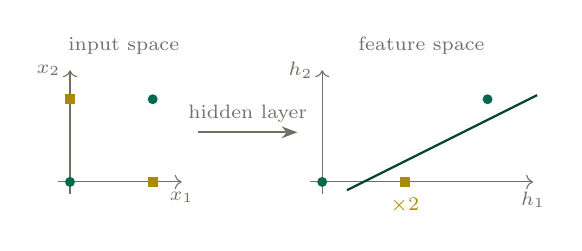
\begin{tikzpicture}[scale=1.05,every node/.style={font=\scriptsize}]
\draw[->,gry] (-0.15,0) -- (1.35,0) node[below]{$x_1$};
\draw[->,gry] (0,-0.15) -- (0,1.35) node[left]{$x_2$};
\fill[acc] (0,0) circle (0.06); \fill[acc] (1,1) circle (0.06);
\fill[gld] (0.94,-0.06) rectangle (1.06,0.06); \fill[gld] (-0.06,0.94) rectangle (0.06,1.06);
\node[text=gry] at (0.65,1.65) {input space};
\draw[-{Stealth[length=2mm]},thick,gry] (1.55,0.6) -- node[above]{hidden layer} (2.75,0.6);
\begin{scope}[xshift=3.05cm]
\draw[->,gry] (-0.15,0) -- (2.55,0) node[below]{$h_1$};
\draw[->,gry] (0,-0.15) -- (0,1.35) node[left]{$h_2$};
\draw[tea,thick] (0.3,-0.1) -- (2.6,1.05);
\fill[acc] (0,0) circle (0.06);
\fill[acc] (2,1) circle (0.06);
\fill[gld] (0.94,-0.06) rectangle (1.06,0.06);
\node[below,text=gld] at (1,-0.08) {$\times2$};
\node[text=gry] at (1.2,1.65) {feature space};
\end{scope}
\end{tikzpicture}
\end{center}

\end{column}
\end{columns}
\vspace{-0.6em}
{\small\[
\begin{array}{c|c|c|c|c}
x & s=x_1+x_2 & h_1=s & h_2=\relu(s-1) & g=h_1-2h_2\\\hline
00 & 0 & 0 & 0 & 0\\
10 & 1 & 1 & 0 & 1\\
01 & 1 & 1 & 0 & 1\\
11 & 2 & 2 & 1 & \mathbf{0}
\end{array}
\]}
\vspace{-0.4em}
\begin{bxrem}
$g(x)=w_2^\top\relu(W_1x+b_1)+b_2$:\ affine $\to$ activation $\to$ affine $=$ the $\FFN$ of every decoder layer.
\end{bxrem}
\end{frame}

% ---------- Expressivity vs trainability -----------------------------
\begin{frame}[t]{Expressivity vs.\ trainability}
\begin{columns}[T]
\begin{column}{0.57\textwidth}
\cfix
\begin{center}
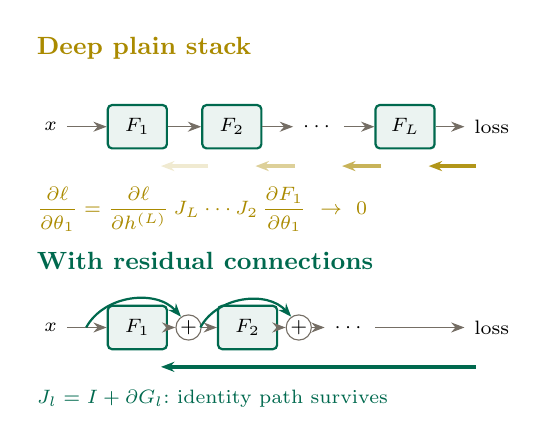
\begin{tikzpicture}[every node/.style={font=\scriptsize},>={Stealth[length=1.7mm]},
  L/.style={blk=acc,minimum width=0.75cm,minimum height=0.55cm}]
\node[font=\small\bfseries,text=gld,anchor=west] at (-0.3,1.0) {Deep plain stack};
\node (x) at (0,0) {$x$};
\node[L] (a1) at (1.1,0) {$F_1$}; \node[L] (a2) at (2.3,0) {$F_2$};
\node (ad) at (3.4,0) {$\cdots$}; \node[L] (aL) at (4.5,0) {$F_L$};
\node (al) at (5.6,0) {loss};
\draw[->,gry] (x)--(a1); \draw[->,gry] (a1)--(a2); \draw[->,gry] (a2)--(ad); \draw[->,gry] (ad)--(aL); \draw[->,gry] (aL)--(al);
\foreach \xa/\xb/\op in {5.4/4.8/90,4.2/3.7/65,3.1/2.6/40,2.0/1.4/18}
  \draw[->,gld!\op,very thick] (\xa,-0.5) -- (\xb,-0.5);
\node[text=gld,anchor=west] at (-0.3,-1.05) {$\dfrac{\partial\ell}{\partial\theta_1}=\dfrac{\partial\ell}{\partial h^{(L)}}\,J_L\cdots J_2\,\dfrac{\partial F_1}{\partial\theta_1}\ \to\ 0$};
\begin{scope}[yshift=-2.55cm]
\node[font=\small\bfseries,text=acc,anchor=west] at (-0.3,0.85) {With residual connections};
\node (y) at (0,0) {$x$};
\node[L] (b1) at (1.1,0) {$F_1$}; \node[circle,draw=gry,inner sep=0pt,minimum size=3.2mm] (s1) at (1.75,0) {$+$};
\node[L] (b2) at (2.5,0) {$F_2$}; \node[circle,draw=gry,inner sep=0pt,minimum size=3.2mm] (s2) at (3.15,0) {$+$};
\node (bd) at (3.8,0) {$\cdots$}; \node (bl) at (5.6,0) {loss};
\draw[->,gry] (y)--(b1); \draw[->,gry] (b1)--(s1); \draw[->,gry] (s1)--(b2); \draw[->,gry] (b2)--(s2); \draw[->,gry] (s2)--(bd); \draw[->,gry] (bd)--(bl);
\draw[->,acc,thick] (0.45,0) to[bend left=55] (s1);
\draw[->,acc,thick] (1.9,0) to[bend left=55] (s2);
\draw[->,acc,very thick] (5.4,-0.5) -- (1.4,-0.5);
\node[text=acc,anchor=west] at (-0.3,-0.9) {$J_l=I+\partial G_l$:\ identity path survives};
\end{scope}
\end{tikzpicture}
\end{center}
\end{column}
\begin{column}{0.41\textwidth}
\cfix
\begin{center}
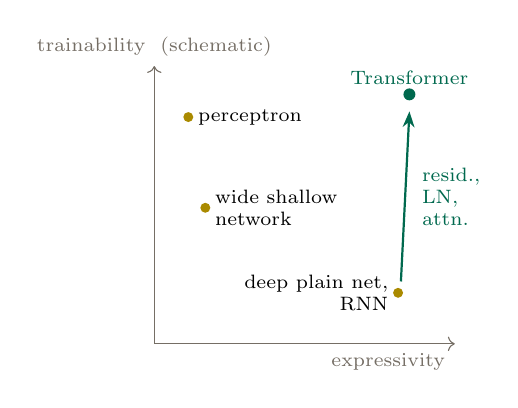
\begin{tikzpicture}[scale=0.72,every node/.style={font=\scriptsize}]
\draw[->,gry] (0,0) -- (5.3,0) node[below left]{expressivity};
\draw[->,gry] (0,0) -- (0,4.9) node[above]{trainability \ (schematic)};
\fill[gld] (0.6,4.0) circle (2.5pt) node[right,text=black,align=left]{perceptron};
\fill[gld] (0.9,2.4) circle (2.5pt) node[right,text=black,align=left]{wide shallow\\network};
\fill[gld] (4.3,0.9) circle (2.5pt) node[left,text=black,align=right]{deep plain net,\\RNN};
\fill[acc] (4.5,4.4) circle (3pt) node[above,text=acc]{Transformer};
\draw[-{Stealth[length=2mm]},acc,thick] (4.35,1.1) -- (4.5,4.1);
\node[text=acc,align=left,anchor=west] at (4.55,2.6) {resid.,\\LN,\\attn.};
\end{tikzpicture}
\end{center}
\end{column}
\end{columns}
\begin{bxrem}
\footnotesize\textbf{Expressivity:} functions the network can represent ($\uparrow$ with $L$).\quad \textbf{Trainability:} gradient descent finds good $\theta$.\\
$L\uparrow\ \Rightarrow$ longer product $J_L\cdots J_{l+1}$, $J_l=\partial F_l/\partial h^{(l-1)}$ $\Rightarrow$ $\partial\ell/\partial\theta_l\to0$ $\Rightarrow$ trainability $\downarrow$. \ Fix: residual $\oplus$ $+$ $\LN$.
\end{bxrem}
\end{frame}

%==================================================
\section{The decoder as maps}

% ---------- Tokens to U ----------------------------------------------
\begin{frame}[t]{$\Emb$, step by step: from tokens to $U^{(0)}$}
\setbeamerfont{itemize/enumerate body}{size=\footnotesize}
\begin{columns}[T]
\begin{column}{0.52\textwidth}
\cfix
\begin{bxdef}
\footnotesize
\begin{enumerate}\setlength{\itemsep}{1pt}
\item[1.] \textbf{Tokenise.} Text $\to$ tokens with ids in $\Vc=\{1,\dots,|\Vc|\}$. Toy model: characters ($|\Vc|=37$); LLMs: subword pieces ($|\Vc|\sim10^4$--$10^5$).
\item[2.] \textbf{One-hot.} $y_i\ \mapsto\ e_{y_i}\in\{0,1\}^{|\Vc|}$, with a $1$ at entry $y_i$.
\item[3.] \textbf{Look up.} $E_{y_i}=E\,e_{y_i}$ = column $y_i$ of $E\in\R^{d\times|\Vc|}$ (in code: a table lookup).
\item[4.] \textbf{Add the position.} $u_i=E_{y_i}+P_i$, \ $P_i=P\,e_i$, \ $e_i\in\{0,1\}^{n_{\rm ctx}}$.
\item[5.] \textbf{Stack.} Row $i$ of $U^{(0)}\in\R^{n\times d}$ is $u_i^\top$.
\end{enumerate}
{\footnotesize\[
U^{(0)}=\Emb(y_1,\dots,y_n)=\begin{pmatrix}(E_{y_1}+P_1)^\top\\[-2pt]\vdots\\(E_{y_n}+P_n)^\top\end{pmatrix}.
\]}
\end{bxdef}
\end{column}
\begin{column}{0.45\textwidth}
\cfix
\begin{center}
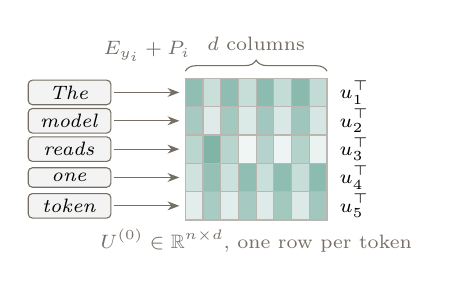
\begin{tikzpicture}[scale=0.75,every node/.style={font=\scriptsize},>={Stealth[length=1.5mm]}]
\node[text=gry] at (0.95,0.45) {$E_{y_i}+P_i$};
\foreach \r/\t in {1/The,2/model,3/reads,4/one,5/token}{
  \node[draw=gry,rounded corners=1.5pt,fill=gry!8,minimum width=1.05cm,inner sep=2pt,anchor=east] (t\r) at (0.35,{-0.48*\r+0.24}) {\textit{\t}};
  \draw[->,gry] (0.4,{-0.48*\r+0.24}) -- (1.5,{-0.48*\r+0.24});
  \foreach \k in {0,...,7}{
    \pgfmathtruncatemacro{\sh}{mod(\r*37+\k*23,45)+6}
    \draw[gry!50,fill=acc!\sh] ({1.6+0.3*\k},{-0.48*\r}) rectangle ({1.6+0.3*(\k+1)},{-0.48*(\r-1)});
  }
  \node[anchor=west] at (4.05,{-0.48*\r+0.24}) {$u_{\r}^\top$};
}
\draw[decorate,decoration={brace,amplitude=4pt},gry] (1.6,0.12) -- node[above=4pt]{$d$ columns} (4.0,0.12);
\node[text=gry] at (2.8,-2.75) {$U^{(0)}\in\R^{n\times d}$, one row per token};
\end{tikzpicture}
\end{center}
\begin{bxrem}
\footnotesize\textbf{Positions.} Trained $P\in\R^{d\times n_{\rm ctx}}$:
\begin{gather*}
P=\big[\,P_1\,\big|\cdots\big|\,P_{n_{\rm ctx}}\big]\\
P_i=P\,e_i\in\R^d,\ \ e_i\in\{0,1\}^{n_{\rm ctx}}
\end{gather*}
$P_i$ = learned vector of position $i$; entries start $\sim\mathcal N(0,0.1^2)$.
\end{bxrem}
\end{column}
\end{columns}
\end{frame}

% ---------- The decoder layer ----------------------------------------
\begin{frame}[t]{The decoder-only architecture}
\begin{columns}[T]
\begin{column}{0.55\textwidth}
\cfix
\begin{bxdef}
Each map below is $\R^{n\times d}\to\R^{n\times d}$:
\begin{align*}
\DL(U)&=\FFNB\big(\AttnB(U)\big)\\
\AttnB(U)&=\LN\big(U+\MHA_M(U)\big)\\
\FFNB(U)&=\LN\big(U+\FFN(U)\big)
\end{align*}
\end{bxdef}
{\small $\DL_1,\dots,\DL_L$: same form, separate parameters.\par}
\end{column}
\begin{column}{0.42\textwidth}
\cfix
\begin{center}
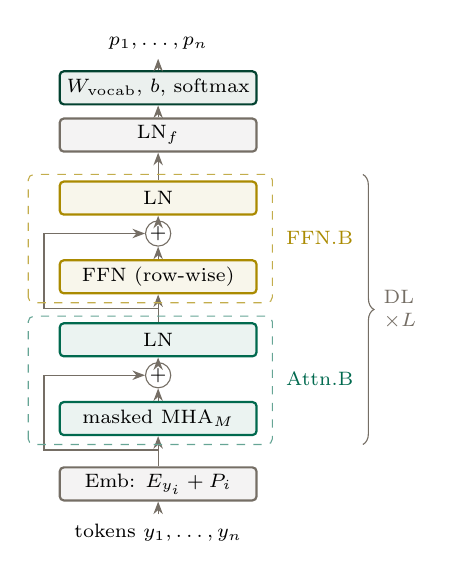
\begin{tikzpicture}[every node/.style={font=\scriptsize},>={Stealth[length=1.6mm]},
  pl/.style={circle,draw=gry,inner sep=0pt,minimum size=3.2mm}]
\node (in) at (0,0) {tokens $y_1,\dots,y_n$};
\node[blkA=gry] (emb) at (0,0.62) {$\Emb$: $E_{y_i}+P_i$};
\node[blkA=acc] (mha) at (0,1.45) {masked $\MHA_M$};
\node[pl] (p1) at (0,2.0) {$+$};
\node[blkA=acc] (ln1) at (0,2.45) {$\LN$};
\node[blkA=gld] (ffn) at (0,3.25) {$\FFN$ (row-wise)};
\node[pl] (p2) at (0,3.8) {$+$};
\node[blkA=gld] (ln2) at (0,4.25) {$\LN$};
\node[blkA=gry] (lnf) at (0,5.05) {$\LN_f$};
\node[blkA=tea] (hd) at (0,5.65) {$\Wv$, $b$, softmax};
\node (out) at (0,6.22) {$p_1,\dots,p_n$};
\draw[->,gry] (in)--(emb); \draw[->,gry] (emb)--(mha); \draw[->,gry] (mha)--(p1); \draw[->,gry] (p1)--(ln1);
\draw[->,gry] (ln1)--(ffn); \draw[->,gry] (ffn)--(p2); \draw[->,gry] (p2)--(ln2); \draw[->,gry] (ln2)--(lnf);
\draw[->,gry] (lnf)--(hd); \draw[->,gry] (hd)--(out);
\draw[->,gry] (0,1.05) -- (-1.45,1.05) -- (-1.45,2.0) -- (p1);
\draw[->,gry] (0,2.85) -- (-1.45,2.85) -- (-1.45,3.8) -- (p2);
\draw[acc!60,dashed,rounded corners=2pt] (-1.65,1.12) rectangle (1.45,2.75);
\draw[gld!70,dashed,rounded corners=2pt] (-1.65,2.92) rectangle (1.45,4.55);
\node[anchor=west,text=acc] at (1.5,1.95) {$\AttnB$};
\node[anchor=west,text=gld] at (1.5,3.75) {$\FFNB$};
\draw[decorate,decoration={brace,amplitude=4pt},gry] (2.6,4.55) -- node[right=4pt,align=left]{$\DL$\\$\times L$} (2.6,1.12);
\end{tikzpicture}
\end{center}
\end{column}
\end{columns}
\end{frame}

%==================================================
\section{Attention block}

\crumbsA{1}
\begin{frame}[t]{$\AttnB$: the block}
\begin{bxdef}
\[
\AttnB:\R^{n\times d}\to\R^{n\times d},\qquad \AttnB(U)=\LN\big(U+\MHA_M(U)\big)
\]
\end{bxdef}
\vspace{0.6em}
\begin{center}
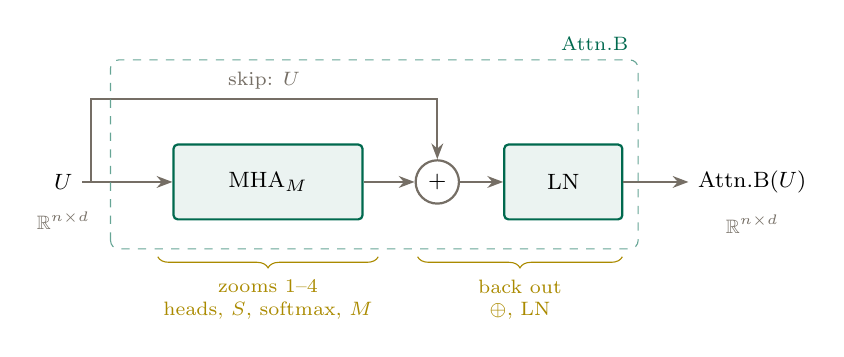
\begin{tikzpicture}[every node/.style={font=\footnotesize},>={Stealth[length=2mm]}]
\node (U) at (0,0) {$U$};
\node[blk=acc,minimum width=2.4cm,minimum height=0.95cm] (m) at (2.6,0) {$\MHA_M$};
\node[circle,draw=gry,thick,inner sep=0pt,minimum size=5.5mm] (pl) at (4.75,0) {$+$};
\node[blk=acc,minimum width=1.5cm,minimum height=0.95cm] (ln) at (6.35,0) {$\LN$};
\node (o) at (8.75,0) {$\AttnB(U)$};
\draw[->,gry,thick] (U)--(m);
\draw[->,gry,thick] (m)--(pl);
\draw[->,gry,thick] (pl)--(ln); \draw[->,gry,thick] (ln)--(o);
\node[text=gry,font=\scriptsize,below=1pt] at (U.south) {$\R^{n\times d}$};
\node[text=gry,font=\scriptsize,below=1pt] at (o.south) {$\R^{n\times d}$};
\draw[->,gry,thick] (0.35,0) -- (0.35,1.05) -- node[above,text=gry,font=\scriptsize]{skip: $U$} (4.75,1.05) -- (pl);
\draw[acc!60,dashed,rounded corners=3pt] (0.6,-0.85) rectangle (7.3,1.55);
\node[text=acc,anchor=south east,font=\scriptsize] at (7.3,1.55) {$\AttnB$};
\draw[decorate,decoration={brace,mirror,amplitude=4pt},gld] (1.2,-0.95) -- node[below=5pt,text=gld,align=center,font=\scriptsize]{zooms 1--4\\heads, $S$, softmax, $M$} (4.0,-0.95);
\draw[decorate,decoration={brace,mirror,amplitude=4pt},gld] (4.5,-0.95) -- node[below=5pt,text=gld,align=center,font=\scriptsize]{back out\\$\oplus$, $\LN$} (7.1,-0.95);
\end{tikzpicture}
\end{center}
\end{frame}

\crumbsA{2}
\begin{frame}[t]{Zoom 1: $\MHA_M$ = heads + concat}
\begin{bxdef}
$h$ heads, $d_k=d/h$. Trained: $W^r_{Q},W^r_K,W^r_V\in\R^{d\times d_k}$ ($r=1,\dots,h$) and $W_O\in\R^{hd_k\times d}$. Fixed: the causal mask $M$. The map $\MHA_M:\R^{n\times d}\to\R^{n\times d}$ is
\[
\MHA_M(U)=\underbrace{\Concat\big(\Attn^M_1(U),\dots,\Attn^M_h(U)\big)}_{\in\,\R^{n\times hd_k}}\,W_O .
\]
\end{bxdef}
\begin{center}
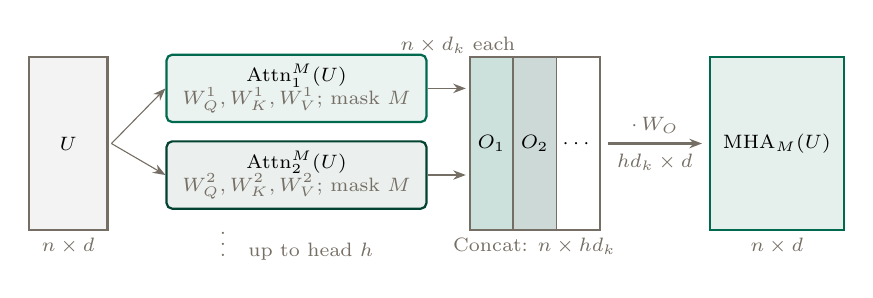
\begin{tikzpicture}[every node/.style={font=\scriptsize},>={Stealth[length=1.6mm]}]
\draw[gry,thick,fill=gry!8] (0,0.2) rectangle (1.0,2.4); \node at (0.5,1.3) {$U$};
\node[text=gry] at (0.5,0) {$n\times d$};
\node[hb=acc] (h1) at (3.4,2.0) {$\Attn^M_1(U)$\\[-1pt]{\color{gry}$W_Q^1,W_K^1,W_V^1$; mask $M$}};
\node[hb=tea] (h2) at (3.4,0.9) {$\Attn^M_2(U)$\\[-1pt]{\color{gry}$W_Q^2,W_K^2,W_V^2$; mask $M$}};
\node[text=gry] at (3.4,0.1) {$\vdots$\quad up to head $h$};
\draw[->,gry] (1.05,1.3) -- (h1.west); \draw[->,gry] (1.05,1.3) -- (h2.west);
\node[text=gry] at (5.45,2.55) {$n\times d_k$ each};
\fill[acc!20] (5.6,0.2) rectangle (6.15,2.4); \fill[tea!20] (6.15,0.2) rectangle (6.7,2.4);
\draw[gry,thick] (5.6,0.2) rectangle (7.25,2.4); \draw[gry] (6.15,0.2) -- (6.15,2.4); \draw[gry] (6.7,0.2) -- (6.7,2.4);
\node at (5.875,1.3) {$O_1$}; \node at (6.425,1.3) {$O_2$}; \node at (6.975,1.3) {$\cdots$};
\draw[->,gry] (h1.east) -- (5.55,2.0); \draw[->,gry] (h2.east) -- (5.55,0.9);
\node[text=gry] at (6.42,0) {Concat: $n\times hd_k$};
\draw[->,thick,gry] (7.35,1.3) -- node[above]{$\cdot\,W_O$} node[below,text=gry]{$hd_k\times d$} (8.55,1.3);
\draw[acc,thick,fill=acc!10] (8.65,0.2) rectangle (10.35,2.4); \node at (9.5,1.3) {$\MHA_M(U)$};
\node[text=gry] at (9.5,0) {$n\times d$};
\end{tikzpicture}
\end{center}
{\small $hd_k=d\ \Rightarrow\ \MHA_M(U)\in\R^{n\times d}$.}
\end{frame}

\crumbsA{3}
\begin{frame}[t]{Zoom 2: one head $\Attn^M_r$}
\begin{bxdef}
Head $r\in\{1,\dots,h\}$. Trained: $W_Q^r,W_K^r,W_V^r\in\R^{d\times d_k}$, giving $Q=UW_Q^r$, $K=UW_K^r$, $V=UW_V^r\in\R^{n\times d_k}$. Fixed: the mask $M\in\{0,-\infty\}^{n\times n}$.
\[
\Attn^M_r:\R^{n\times d}\to\R^{n\times d_k},\qquad
\Attn^M_r(U)=\underbrace{\softmax_{\rm row}\!\Big(\frac{QK^\top}{\sqrt{d_k}}+M\Big)}_{A\,\in\,\R^{n\times n}}V
\]
\end{bxdef}
\vspace{-0.3em}
\begin{center}
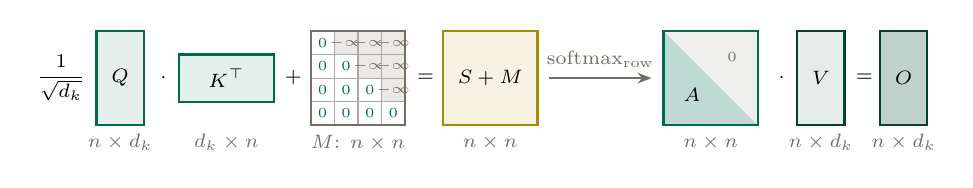
\begin{tikzpicture}[every node/.style={font=\scriptsize},>={Stealth[length=1.8mm]}]
\def\uu{0.3}
% 1/sqrt(dk) Q K^T
\node at (-0.45,2*\uu) {$\dfrac{1}{\sqrt{d_k}}$};
\draw[acc,thick,fill=acc!10] (0,0) rectangle (2*\uu,4*\uu); \node at (\uu,2*\uu) {$Q$};
\node[text=gry] at (\uu,-0.22) {$n\times d_k$};
\node at (0.85,2*\uu) {$\cdot$};
\draw[acc,thick,fill=acc!10] (1.05,\uu) rectangle (1.05+4*\uu,3*\uu); \node at (1.05+2*\uu,2*\uu) {$K^\top$};
\node[text=gry] at (1.05+2*\uu,-0.22) {$d_k\times n$};
\node at (2.5,2*\uu) {$+$};
% M: 0 on/below diagonal, -inf above
\begin{scope}[xshift=2.72cm]
\foreach \i in {1,...,4}{\foreach \j in {1,...,4}{
  \ifnum\j>\i
    \draw[gry!60,fill=gry!15] ({\uu*(\j-1)},{\uu*(4-\i)}) rectangle ({\uu*\j},{\uu*(5-\i)});
    \node[text=gry,font=\fontsize{4.5}{5}\selectfont] at ({\uu*(\j-0.5)},{\uu*(4.5-\i)}) {$-\infty$};
  \else
    \draw[gry!60,fill=white] ({\uu*(\j-1)},{\uu*(4-\i)}) rectangle ({\uu*\j},{\uu*(5-\i)});
    \node[text=acc,font=\tiny] at ({\uu*(\j-0.5)},{\uu*(4.5-\i)}) {$0$};
  \fi}}
\draw[gry,thick] (0,0) rectangle (4*\uu,4*\uu);
\node[text=gry] at (2*\uu,-0.22) {$M$: $n\times n$};
\end{scope}
\node at (4.18,2*\uu) {$=$};
\draw[gld,thick,fill=gld!10] (4.4,0) rectangle (4.4+4*\uu,4*\uu); \node at (4.4+2*\uu,2*\uu) {$S+M$};
\node[text=gry] at (4.4+2*\uu,-0.22) {$n\times n$};
\draw[->,thick,gry] (5.75,2*\uu) -- node[above]{$\softmax_{\rm row}$} (7.05,2*\uu);
\fill[acc!25] (7.2,4*\uu) -- (7.2,0) -- (7.2+4*\uu,0) -- cycle;
\fill[gry!12] (7.2,4*\uu) -- (7.2+4*\uu,4*\uu) -- (7.2+4*\uu,0) -- cycle;
\draw[acc,thick] (7.2,0) rectangle (7.2+4*\uu,4*\uu); \node at (7.2+1.2*\uu,1.3*\uu) {$A$};
\node[text=gry,font=\tiny] at (7.2+2.9*\uu,2.9*\uu) {$0$};
\node[text=gry] at (7.2+2*\uu,-0.22) {$n\times n$};
\node at (8.7,2*\uu) {$\cdot$};
\draw[tea,thick,fill=tea!10] (8.9,0) rectangle (8.9+2*\uu,4*\uu); \node at (8.9+\uu,2*\uu) {$V$};
\node[text=gry] at (8.9+\uu,-0.22) {$n\times d_k$};
\node at (9.75,2*\uu) {$=$};
\draw[tea,thick,fill=tea!25] (9.95,0) rectangle (9.95+2*\uu,4*\uu); \node at (9.95+\uu,2*\uu) {$O$};
\node[text=gry] at (9.95+\uu,-0.22) {$n\times d_k$};
\end{tikzpicture}
\end{center}
\vspace{-0.4em}
{\small\textbf{Row view.} $o_i=\sum_{j}a_{ij}\,v_j$, \ $a_{i\cdot}\in\Delta^{n-1}$, \ so \ $o_i\in\operatorname{conv}\{v_j:\ M_{ij}=0\}=\operatorname{conv}\{v_1,\dots,v_i\}$,\\[2pt]
where $\Delta^{n-1}=\big\{a\in\R^n:\ a_j\ge0\ \text{for all } j,\ \sum_{j=1}^n a_j=1\big\}\subset\R^n$.\par}
{\footnotesize\color{tea}\textbf{Statistician's reading:} Nadaraya--Watson smoothing of the $v_j$ with kernel $\kappa(q_i,k_j)=\exp\big(q_i^\top k_j/\sqrt{d_k}\big)$.\par}
\end{frame}

\crumbsA{4}
\begin{frame}[t]{Zoom 3: scores and softmax}
\begin{bxdef}
\[
S=\frac{QK^\top}{\sqrt{d_k}}\in\R^{n\times n},\quad s_{ij}=\frac{q_i^\top k_j}{\sqrt{d_k}};\qquad
a_{i\cdot}=\softmax\big(s_{i\cdot}+M_{i\cdot}\big)\in\Delta^{n-1}\subset\R^n
\]
\[
\softmax:\R^n\to\Delta^{n-1},\qquad \softmax(z)_j=\frac{e^{z_j}}{\sum_{k}e^{z_k}}\in\R
\]
\end{bxdef}
\begin{center}
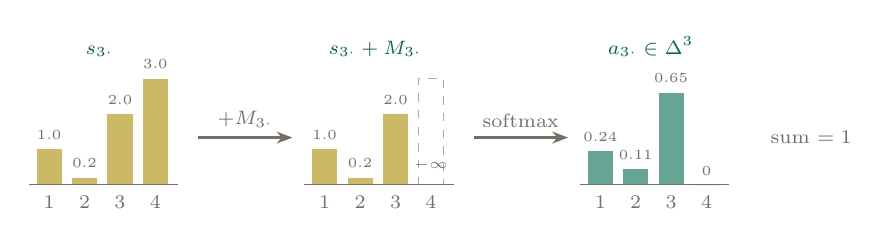
\begin{tikzpicture}[every node/.style={font=\scriptsize},>={Stealth[length=2mm]}]
% panel 1: scores of row i=3
\node[text=acc,anchor=south] at (0.8,1.5) {$s_{3\cdot}$};
\foreach \j/\v in {1/1.0,2/0.2,3/2.0,4/3.0}{
  \fill[gld!60] ({0.45*(\j-1)},0) rectangle ({0.45*(\j-1)+0.32},{0.45*\v});
  \node[text=gry,anchor=south,font=\tiny] at ({0.45*(\j-1)+0.16},{0.45*\v}) {\v};
  \node[text=gry] at ({0.45*(\j-1)+0.16},-0.22) {$\j$};}
\draw[gry] (-0.1,0) -- (1.8,0);
\draw[->,thick,gry] (2.05,0.6) -- node[above]{$+M_{3\cdot}$} (3.25,0.6);
% panel 2: masked
\begin{scope}[xshift=3.5cm]
\node[text=acc,anchor=south] at (0.8,1.5) {$s_{3\cdot}+M_{3\cdot}$};
\foreach \j/\v in {1/1.0,2/0.2,3/2.0}{
  \fill[gld!60] ({0.45*(\j-1)},0) rectangle ({0.45*(\j-1)+0.32},{0.45*\v});
  \node[text=gry,anchor=south,font=\tiny] at ({0.45*(\j-1)+0.16},{0.45*\v}) {\v};
  \node[text=gry] at ({0.45*(\j-1)+0.16},-0.22) {$\j$};}
\draw[gry!60,dashed] (1.35,0) rectangle (1.67,1.35);
\node[text=gry,font=\tiny] at (1.51,0.25) {$-\infty$};
\node[text=gry] at (1.51,-0.22) {$4$};
\draw[gry] (-0.1,0) -- (1.8,0);
\end{scope}
\draw[->,thick,gry] (5.55,0.6) -- node[above]{$\softmax$} (6.75,0.6);
% panel 3: weights
\begin{scope}[xshift=7.0cm]
\node[text=acc,anchor=south] at (0.8,1.5) {$a_{3\cdot}\in\Delta^{3}$};
\foreach \j/\v in {1/0.24,2/0.11,3/0.65,4/0}{
  \fill[acc!60] ({0.45*(\j-1)},0) rectangle ({0.45*(\j-1)+0.32},{1.8*\v});
  \node[text=gry,anchor=south,font=\tiny] at ({0.45*(\j-1)+0.16},{1.8*\v}) {\v};
  \node[text=gry] at ({0.45*(\j-1)+0.16},-0.22) {$\j$};}
\draw[gry] (-0.1,0) -- (1.8,0);
\end{scope}
\node[text=gry,anchor=west] at (9.2,0.6) {sum $=1$};
\end{tikzpicture}
\end{center}
\begin{bxthm}
\small $\softmax(z+c\one)=\softmax(z)$;\quad $z_j=-\infty\Rightarrow\softmax(z)_j=0$.
\end{bxthm}
\end{frame}

\crumbsA{5}
\begin{frame}[t]{Zoom 4: why the mask $M$}
\begin{columns}[T]
\begin{column}{0.57\textwidth}
{\small Training window: $y=(y_1,\dots,y_{n+1})$, input $y_{1:n}$, and position $i$ is scored by $L_i=-\log p_i[y_{i+1}]$.\par\vspace{0.3em}
Without a mask, row $i$ of $\MHA$ (no mask) sees $u_{i+1}=E_{y_{i+1}}+P_{i+1}$, which \emph{contains the answer}. A minimiser can copy it, so $L_i\to0$ and nothing about language is learned.\par}
\begin{bxdef}
\textbf{Causal mask.} $M\in\{0,-\infty\}^{n\times n}$ with $M_{ij}=0$ for $j\le i$ and $M_{ij}=-\infty$ for $j>i$. With $s_{ij}=q_i^\top k_j/\sqrt{d_k}$:
\[
a_{ij}=\frac{e^{s_{ij}}}{\sum_{j'\le i}e^{s_{ij'}}}\ \ (j\le i),
\]
and $a_{ij}=0$ for $j>i$.
\end{bxdef}
\end{column}
\begin{column}{0.4\textwidth}
\cfix
\begin{center}
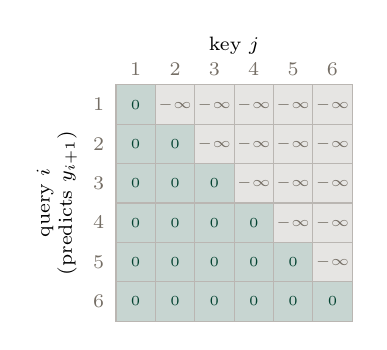
\begin{tikzpicture}[every node/.style={font=\tiny}]
\def\c{0.5}
\foreach \i in {1,...,6}{
  \foreach \j in {1,...,6}{
    \ifnum\j>\i
      \draw[gry!50,fill=gry!18] ({\c*(\j-1)},{-\c*\i}) rectangle ({\c*\j},{-\c*(\i-1)});
      \node[text=gry] at ({\c*(\j-0.5)},{-\c*(\i-0.5)}) {$-\infty$};
    \else
      \draw[gry!50,fill=tea!22] ({\c*(\j-1)},{-\c*\i}) rectangle ({\c*\j},{-\c*(\i-1)});
      \node[text=tea] at ({\c*(\j-0.5)},{-\c*(\i-0.5)}) {$0$};
    \fi
  }
  \node[text=gry,font=\scriptsize] at (-0.22,{-\c*(\i-0.5)}) {\i};
  \node[text=gry,font=\scriptsize] at ({\c*(\i-0.5)},0.2) {\i};
}
\node[font=\scriptsize,rotate=90,align=center] at (-0.75,{-3*\c}) {query $i$\\(predicts $y_{i+1}$)};
\node[font=\scriptsize] at ({3*\c},0.5) {key $j$};
\end{tikzpicture}
\end{center}
{\footnotesize $M$ is part of $\pi_\theta$: used in training and at inference.\par}
\end{column}
\end{columns}
\end{frame}

\crumbsA{5}
\begin{frame}[t]{Zoom 4: $\Attn$ vs.\ $\Attn^M$}
\begin{columns}[T]
\begin{column}{0.48\textwidth}
\cfix
\begin{bxdef}
\scriptsize $\Attn_r(U)=\softmax_{\rm row}\big(QK^\top/\sqrt{d_k}\big)V$
\end{bxdef}
\begin{center}
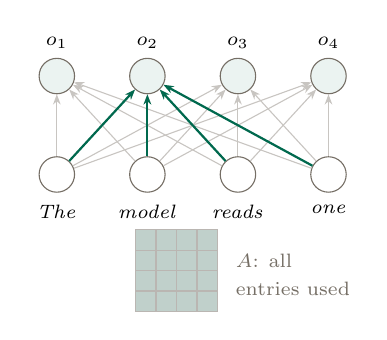
\begin{tikzpicture}[every node/.style={font=\scriptsize},>={Stealth[length=1.3mm]},
  nd/.style={circle,draw=gry,minimum size=4.5mm,inner sep=0pt}]
\foreach \i/\t in {1/The,2/model,3/reads,4/one}{
  \node[nd] (b\i) at ({1.15*(\i-1)},0) {}; \node[below=1pt] at (b\i.south) {\textit{\t}};
  \node[nd,fill=acc!8] (o\i) at ({1.15*(\i-1)},1.25) {}; \node[above=0pt] at (o\i.north) {$o_\i$};}
\foreach \i in {1,...,4}{\foreach \j in {1,...,4}{\draw[->,gry!40] (b\j)--(o\i);}}
\foreach \j in {1,...,4}{\draw[->,acc,thick] (b\j)--(o2);}
\begin{scope}[xshift=1.0cm,yshift=-0.7cm]
\foreach \i in {1,...,4}{\foreach \j in {1,...,4}{
  \draw[gry!50,fill=tea!25] ({0.26*(\j-1)},{-0.26*\i}) rectangle ({0.26*\j},{-0.26*(\i-1)});}}
\node[anchor=west,text=gry] at (1.15,-0.4) {$A$: all};
\node[anchor=west,text=gry] at (1.15,-0.75) {entries used};
\end{scope}
\end{tikzpicture}
\end{center}
{\small Every token sees every token (\emph{encoders}).}
\end{column}
\begin{column}{0.48\textwidth}
\cfix
\begin{bxdef}
\scriptsize $\Attn^M_r(U)=\softmax_{\rm row}\big(QK^\top/\sqrt{d_k}+M\big)V$
\end{bxdef}
\begin{center}
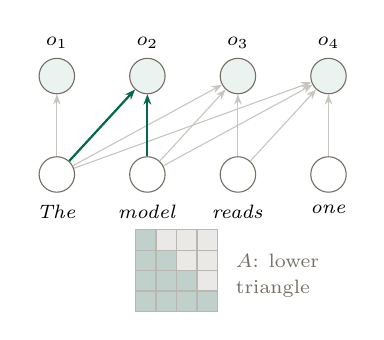
\begin{tikzpicture}[every node/.style={font=\scriptsize},>={Stealth[length=1.3mm]},
  nd/.style={circle,draw=gry,minimum size=4.5mm,inner sep=0pt}]
\foreach \i/\t in {1/The,2/model,3/reads,4/one}{
  \node[nd] (b\i) at ({1.15*(\i-1)},0) {}; \node[below=1pt] at (b\i.south) {\textit{\t}};
  \node[nd,fill=acc!8] (o\i) at ({1.15*(\i-1)},1.25) {}; \node[above=0pt] at (o\i.north) {$o_\i$};}
\foreach \i in {1,...,4}{\foreach \j in {1,...,\i}{\draw[->,gry!40] (b\j)--(o\i);}}
\foreach \j in {1,2}{\draw[->,acc,thick] (b\j)--(o2);}
\begin{scope}[xshift=1.0cm,yshift=-0.7cm]
\foreach \i in {1,...,4}{\foreach \j in {1,...,4}{
  \ifnum\j>\i \draw[gry!50,fill=gry!15] ({0.26*(\j-1)},{-0.26*\i}) rectangle ({0.26*\j},{-0.26*(\i-1)});
  \else \draw[gry!50,fill=tea!25] ({0.26*(\j-1)},{-0.26*\i}) rectangle ({0.26*\j},{-0.26*(\i-1)}); \fi}}
\node[anchor=west,text=gry] at (1.15,-0.4) {$A$: lower};
\node[anchor=west,text=gry] at (1.15,-0.75) {triangle};
\end{scope}
\end{tikzpicture}
\end{center}
{\small Token $i$ sees tokens $1,\dots,i$ (\emph{decoders}).}
\end{column}
\end{columns}
{\footnotesize\color{gry} Decoder-only: no encoder, hence no cross-attention.\par}
\end{frame}

\crumbsA{5}
\begin{frame}[t]{Zoom 4: mask $\Rightarrow p_i=\pi_\theta(\,\cdot\mid y_{\le i})$}
\begin{columns}[T]
\begin{column}{0.6\textwidth}
\cfix
\begin{bxdef}
\small\textbf{Claim.} $p_i=\pi_\theta(\,\cdot\mid y_{\le i})$: \ $p_i$ is a function of $y_{\le i}=(y_1,\dots,y_i)$ only, so $p_i(v)=\P_\theta(y_{i+1}=v\mid y_{\le i})$.
\end{bxdef}
\begin{bxthm}
\small\textbf{Proposition.} With the causal mask $M$, for every layer $l$ and position $i$, row $i$ of $U^{(l)}$ depends only on $y_1,\dots,y_i$. Hence the claim holds.
\end{bxthm}
{\small\textbf{Proof sketch (induction on $l$).} Row $i$ of $U^{(0)}$ is $E_{y_i}+P_i$. In each masked head $\Attn^M_r$, $a_{ij}=0$ for $j>i$, so row $i$ mixes rows $j\le i$ only; the $\oplus$, $\LN$ and $\FFN$ act on each row separately. $\blacksquare$\par\vspace{0.3em}
\textbf{Payoff.} $\sum_{i=1}^n L_i=-\log\pi_\theta(y_{2:n+1}\mid y_1)$.\par}
\end{column}
\begin{column}{0.37\textwidth}
\cfix
\begin{center}
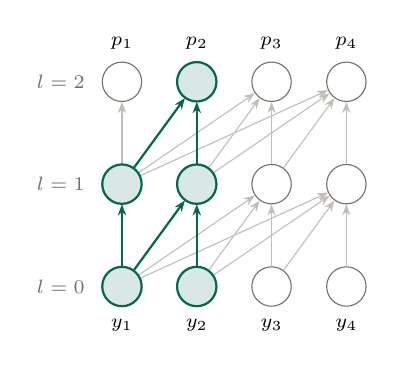
\begin{tikzpicture}[every node/.style={font=\scriptsize},>={Stealth[length=1.4mm]},
  nd/.style={circle,draw=gry,minimum size=5mm,inner sep=0pt}]
\def\dx{0.95}\def\dy{1.3}
\foreach \l in {0,1,2}{\foreach \i in {1,...,4}{\node[nd] (n\l\i) at ({\dx*(\i-1)},{\dy*\l}) {};}}
\foreach \l/\m in {0/1,1/2}{
  \foreach \i in {1,...,4}{\foreach \j in {1,...,\i}{\draw[->,gry!45] (n\l\j) -- (n\m\i);}}}
\foreach \nd in {n01,n02,n11,n12,n22} \node[nd,draw=acc,thick,fill=acc!15] at (\nd) {};
\draw[->,acc,thick] (n01)--(n11); \draw[->,acc,thick] (n01)--(n12); \draw[->,acc,thick] (n02)--(n12);
\draw[->,acc,thick] (n11)--(n22); \draw[->,acc,thick] (n12)--(n22);
\foreach \i in {1,...,4}{\node[below=1pt] at (n0\i.south) {$y_\i$}; \node[above=1pt] at (n2\i.north) {$p_\i$};}
\node[anchor=east,text=gry] at (-0.35,0) {$l=0$};
\node[anchor=east,text=gry] at (-0.35,\dy) {$l=1$};
\node[anchor=east,text=gry] at (-0.35,2*\dy) {$l=2$};
\end{tikzpicture}
\end{center}
{\footnotesize\color{gry} Green: dependencies of $p_2$.\par}
\end{column}
\end{columns}
\end{frame}

\crumbsA{6}
\begin{frame}[t]{Back out: residual $\oplus$ and $\LN$}
\begin{columns}[T]
\begin{column}{0.58\textwidth}
\cfix
\begin{bxdef}
\small\textbf{LayerNorm.} Trained: $\gamma,\beta\in\R^d$. Fixed: a small $\varepsilon>0$. For $u\in\R^d$ let $\mu(u)=\tfrac1d\one^\top u$ and $s^2(u)=\tfrac1d\|u-\mu(u)\one\|^2$. Then $\LN:\R^d\to\R^d$ is
\[
\LN(u)=\gamma\odot\frac{u-\mu(u)\one}{\sqrt{s^2(u)+\varepsilon}}+\beta,
\]
applied to each row of a matrix.\\[4pt]
\textbf{Block.} $\AttnB:\R^{n\times d}\to\R^{n\times d}$,
\[
\AttnB(U)=\LN\big(U+\MHA_M(U)\big).
\]
\end{bxdef}

\end{column}
\begin{column}{0.39\textwidth}
\cfix
\begin{center}
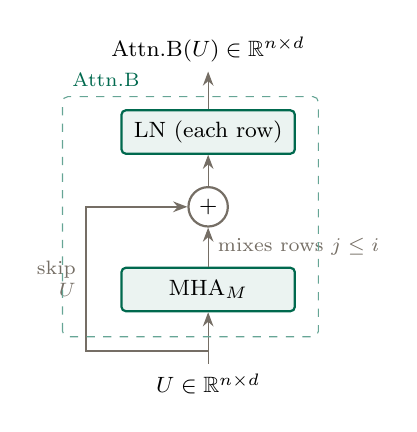
\begin{tikzpicture}[every node/.style={font=\footnotesize},>={Stealth[length=1.8mm]}]
\node (U) at (0,0) {$U\in\R^{n\times d}$};
\node[blkB=acc] (m) at (0,1.2) {$\MHA_M$};
\node[circle,draw=gry,thick,inner sep=0pt,minimum size=5mm] (pl) at (0,2.25) {$+$};
\node[blkB=acc] (ln) at (0,3.2) {$\LN$ (each row)};
\node (o) at (0,4.25) {$\AttnB(U)\in\R^{n\times d}$};
\draw[->,gry] (U)--(m); \draw[->,gry] (m)--node[right,font=\scriptsize,text=gry]{mixes rows $j\le i$}(pl); \draw[->,gry] (pl)--(ln); \draw[->,gry] (ln)--(o);
\draw[->,gry,thick] (0,0.42) -- (-1.55,0.42) -- node[left,font=\scriptsize,text=gry,align=right]{skip\\$U$} (-1.55,2.25) -- (pl);
\draw[acc!60,dashed,rounded corners=2pt] (-1.85,0.6) rectangle (1.4,3.65);
\node[text=acc,anchor=south west,font=\scriptsize] at (-1.85,3.65) {$\AttnB$};
\end{tikzpicture}
\end{center}
{\small Row $i$: rows $j\le i$ enter only via $\MHA_M$; $\oplus$ and $\LN$ act row-wise.}
\end{column}
\end{columns}
\end{frame}

%==================================================
\section{Feed-forward block}

\crumbsF{1}
\begin{frame}[t]{$\FFNB$: the block}
\begin{bxthm}
\scriptsize\textbf{Universal approximation} (Cybenko 1989; Leshno et al.\ 1993). Let $\sigma:\R\to\R$ be continuous and not a polynomial, and let $K\subset\R^p$ be compact. Then the set of one-hidden-layer networks
\[
\mathcal N_\sigma=\Big\{\,g(x)=\sum_{m=1}^{M}c_m\,\sigma\big(a_m^\top x+b_m\big)\ :\ M\in\N,\ a_m\in\R^p,\ b_m,c_m\in\R\Big\}
\]
is dense in $C(K)$ in the sup norm. That is: for every continuous $f:K\to\R$ and every $\varepsilon>0$ there is a $g\in\mathcal N_\sigma$ with
$\sup_{x\in K}|f(x)-g(x)|<\varepsilon$.
\end{bxthm}
\begin{bxdef}
\[
\FFNB:\R^{n\times d}\to\R^{n\times d},\qquad \FFNB(U)=\LN\big(U+\FFN(U)\big)
\]
\end{bxdef}
\begin{center}
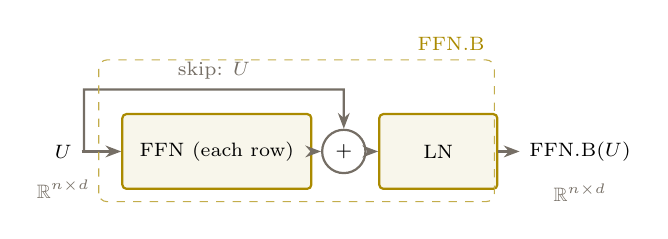
\begin{tikzpicture}[scale=0.75,every node/.style={font=\scriptsize},>={Stealth[length=2mm]}]
\node (U) at (0,0) {$U$};
\node[blk=gld,minimum width=2.4cm,minimum height=0.95cm] (m) at (2.6,0) {$\FFN$ (each row)};
\node[circle,draw=gry,thick,inner sep=0pt,minimum size=5.5mm] (pl) at (4.75,0) {$+$};
\node[blk=gld,minimum width=1.5cm,minimum height=0.95cm] (ln) at (6.35,0) {$\LN$};
\node (o) at (8.75,0) {$\FFNB(U)$};
\draw[->,gry,thick] (U)--(m);
\draw[->,gry,thick] (m)--(pl);
\draw[->,gry,thick] (pl)--(ln); \draw[->,gry,thick] (ln)--(o);
\node[text=gry,font=\scriptsize,below=1pt] at (U.south) {$\R^{n\times d}$};
\node[text=gry,font=\scriptsize,below=1pt] at (o.south) {$\R^{n\times d}$};
\draw[->,gry,thick] (0.35,0) -- (0.35,1.05) -- node[above,text=gry,font=\scriptsize]{skip: $U$} (4.75,1.05) -- (pl);
\draw[gld!70,dashed,rounded corners=3pt] (0.6,-0.85) rectangle (7.3,1.55);
\node[text=gld,anchor=south east,font=\scriptsize] at (7.3,1.55) {$\FFNB$};
\end{tikzpicture}
\end{center}
\end{frame}

\crumbsF{2}
\begin{frame}[t]{Zoom 1: the row-wise lift}
\begin{columns}[T]
\begin{column}{0.52\textwidth}
\cfix
\begin{bxdef}
$U$ with rows $u_1^\top,\dots,u_n^\top$; for one row $u\in\R^d$:
\[
\FFN(u)=W_2\,\sigma(W_1u+b_1)+b_2\in\R^d
\]
Stacked over the rows:
\[
\FFN(U)=\begin{pmatrix}\FFN(u_1)^\top\\[-2pt]\vdots\\\FFN(u_n)^\top\end{pmatrix}\in\R^{n\times d}
\]
Matrix form:
{\small\[
\FFN(U)=\sigma\big(UW_1^\top+\one_nb_1^\top\big)W_2^\top+\one_nb_2^\top
\]}
\end{bxdef}
\end{column}
\begin{column}{0.45\textwidth}
\cfix
\begin{center}
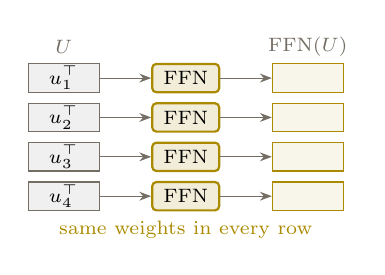
\begin{tikzpicture}[every node/.style={font=\scriptsize},>={Stealth[length=1.5mm]},
  rw/.style={draw=gry,fill=gry!10,minimum width=0.9cm,minimum height=0.36cm,inner sep=0pt},
  fb/.style={draw=gld,thick,fill=gld!15,rounded corners=1.5pt,minimum width=0.85cm,minimum height=0.36cm,inner sep=0pt},
  ob/.style={draw=gld,fill=gld!8,minimum width=0.9cm,minimum height=0.36cm,inner sep=0pt}]
\foreach \i in {1,...,4}{
  \node[rw] (r\i) at (0,{-0.5*\i}) {$u_\i^\top$};
  \node[fb] (f\i) at (1.55,{-0.5*\i}) {$\FFN$};
  \node[ob] (q\i) at (3.1,{-0.5*\i}) {};
  \draw[->,gry] (r\i)--(f\i); \draw[->,gry] (f\i)--(q\i);
}
\node[text=gry] at (0,-0.1) {$U$};
\node[text=gld] at (1.55,-2.42) {same weights in every row};
\node[text=gry] at (3.1,-0.1) {$\FFN(U)$};
\end{tikzpicture}
\end{center}
\end{column}
\end{columns}
\end{frame}

\crumbsF{3}
\begin{frame}[t]{Zoom 2: the map $\FFN(u)$}
\begin{columns}[T]
\begin{column}{0.53\textwidth}
\cfix
\begin{bxdef}
Trained: $W_1\in\R^{\dff\times d}$, $b_1\in\R^{\dff}$, $W_2\in\R^{d\times\dff}$, $b_2\in\R^d$ (typically $\dff=4d$).
Fixed: an activation $\sigma:\R\to\R$, applied entrywise. The map $\FFN:\R^d\to\R^d$ is
\[
\FFN(u)=W_2\,\sigma(W_1u+b_1)+b_2 .
\]
\end{bxdef}
{\small\textbf{Shapes.} $u\in\R^d\ \xrightarrow{\ W_1\cdot+b_1\ }\ \R^{\dff}\ \xrightarrow{\ \sigma\ }\ \R^{\dff}\ \xrightarrow{\ W_2\cdot+b_2\ }\ \R^d$.\par}
\end{column}
\begin{column}{0.44\textwidth}
\cfix
\begin{center}
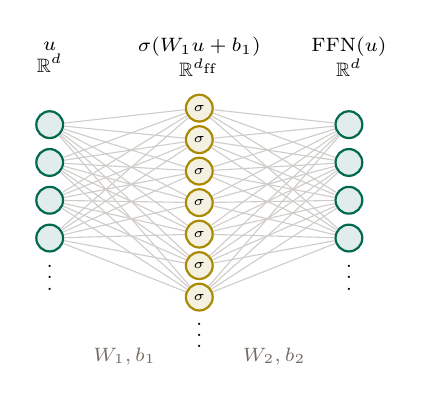
\begin{tikzpicture}[every node/.style={font=\scriptsize},
  ni/.style={circle,draw=acc,thick,fill=acc!12,minimum size=3.4mm,inner sep=0pt},
  nh/.style={circle,draw=gld,thick,fill=gld!12,minimum size=3.4mm,inner sep=0pt,font=\tiny}]
\foreach \k in {1,...,4}{\node[ni] (a\k) at (0,{0.48*(\k-1)+0.75}) {};}
\foreach \k in {1,...,7}{\node[nh] (b\k) at (1.9,{0.4*(\k-1)}) {$\sigma$};}
\foreach \k in {1,...,4}{\node[ni] (c\k) at (3.8,{0.48*(\k-1)+0.75}) {};}
\foreach \p in {1,...,4}{\foreach \q in {1,...,7}{\draw[gry!35] (a\p)--(b\q); \draw[gry!35] (b\q)--(c\p);}}
\node at (0,0.35) {$\vdots$}; \node at (3.8,0.35) {$\vdots$}; \node at (1.9,-0.38) {$\vdots$};
\node[align=center] at (0,3.05) {$u$\\$\R^{d}$};
\node[align=center] at (1.9,3.05) {$\sigma(W_1u+b_1)$\\$\R^{\dff}$};
\node[align=center] at (3.8,3.05) {$\FFN(u)$\\$\R^{d}$};
\node[text=gry] at (0.95,-0.75) {$W_1,b_1$};
\node[text=gry] at (2.85,-0.75) {$W_2,b_2$};
\end{tikzpicture}
\end{center}
\end{column}
\end{columns}
\end{frame}

%==================================================
\crumbsoff
\section{Assembly}

% ---------- Surprise game -----------------------------------------------
\begin{frame}[t]{A game: how surprised are you?}
\begin{center}
{\normalsize \textit{``I am working hard on my physique, so you will find me at the \underline{\hspace{1.8cm}}.''}}
\end{center}
\begin{center}
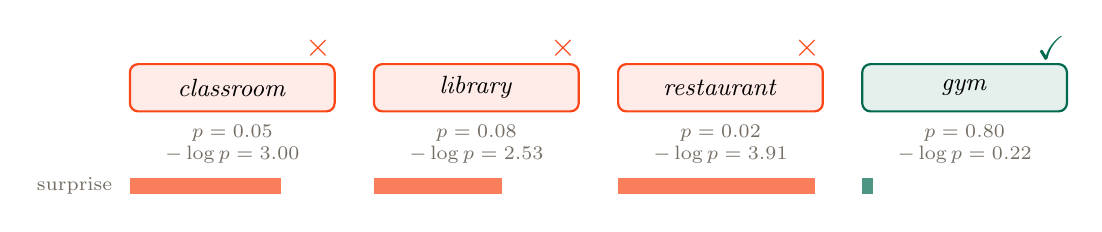
\begin{tikzpicture}[every node/.style={font=\small}]
\def\bw{2.6}
\node[anchor=east,text=gry,font=\scriptsize] at (-1.4,-1.25) {surprise};
\foreach \k/\w/\p/\L/\col/\ok in {0/classroom/0.05/3.00/rust/0,1/library/0.08/2.53/rust/0,2/restaurant/0.02/3.91/rust/0,3/gym/0.80/0.22/acc/1}{
  \pgfmathtruncatemacro{\ov}{\k+2}
  \begin{scope}[xshift={\k*3.1cm},visible on=<\ov->]
  \node[draw=\col,thick,rounded corners=3pt,fill=\col!10,minimum width=\bw cm,minimum height=0.6cm] (w\k) at (0,0) {\textit{\w}};
  \node[text=gry,font=\scriptsize,align=center] at (0,-0.72) {$p=\p$\\$-\log p=\L$};
  \fill[\col!70] ({-\bw/2},-1.35) rectangle ({-\bw/2+0.64*\L},-1.15);
  \ifnum\ok=1 \node[text=acc,font=\large\bfseries] at (1.1,0.5) {\checkmark}; \else \node[text=\col,font=\large\bfseries] at (1.1,0.5) {$\times$}; \fi
  \end{scope}
}
\end{tikzpicture}
\end{center}
\vspace{-0.4em}
\uncover<6->{%
\begin{bxdef}
\footnotesize\textbf{Next: the loss. Its goal.} The loss trains the model to assign, at each position $i$ (token index), a probability $p_i(v)$ to every token $v\in\Vc$ that matches how likely $v$ is to come next given $y_1,\dots,y_i$. \emph{Choosing the next token from $p_i$ (argmax or sampling) is a separate decoding step.}
\end{bxdef}
\vspace{-0.2em}
\begin{bxrem}
\footnotesize $L_i(\theta)$ \textbf{is the surprisal of the true next token.} At parameters $\theta$, the model reads the prefix $y_1,\dots,y_i$ and assigns probability $p_i(y_{i+1})$ to the token that actually comes next. $L_i(\theta)=-\log p_i(y_{i+1})$ measures how surprised it was: near $0$ when the model was confident and right, large when it gave the true token little probability.
\end{bxrem}}
\end{frame}

% ---------- Training loop --------------------------------------------
% ---------- Loss and derivative ---------------------------------------
\begin{frame}[t]{The loss}
\begin{bxdef}
\small
$H=\LN_f\big(U^{(L)}\big)\in\R^{n\times d}$, \ $h_i^\top=$ row $i$ of $H$ \ (final hidden vector at position $i$).
\begin{align*}
z_i&=\Wv^\top h_i+b\in\R^{|\Vc|}, & p_i&=\softmax(z_i)\in\Delta(\Vc),\\
L_i(\theta)&=-\log p_i(y_{i+1})=-z_{i,y_{i+1}}+\log\textstyle\sum_{v\in\Vc}e^{z_{i,v}}, & \ell(\theta)&=\tfrac1{Bn}\textstyle\sum_{s=1}^{B}\sum_{i=1}^{n}L_i^{(s)}(\theta).
\end{align*}
\end{bxdef}
\begin{center}
\resizebox{\textwidth}{!}{%
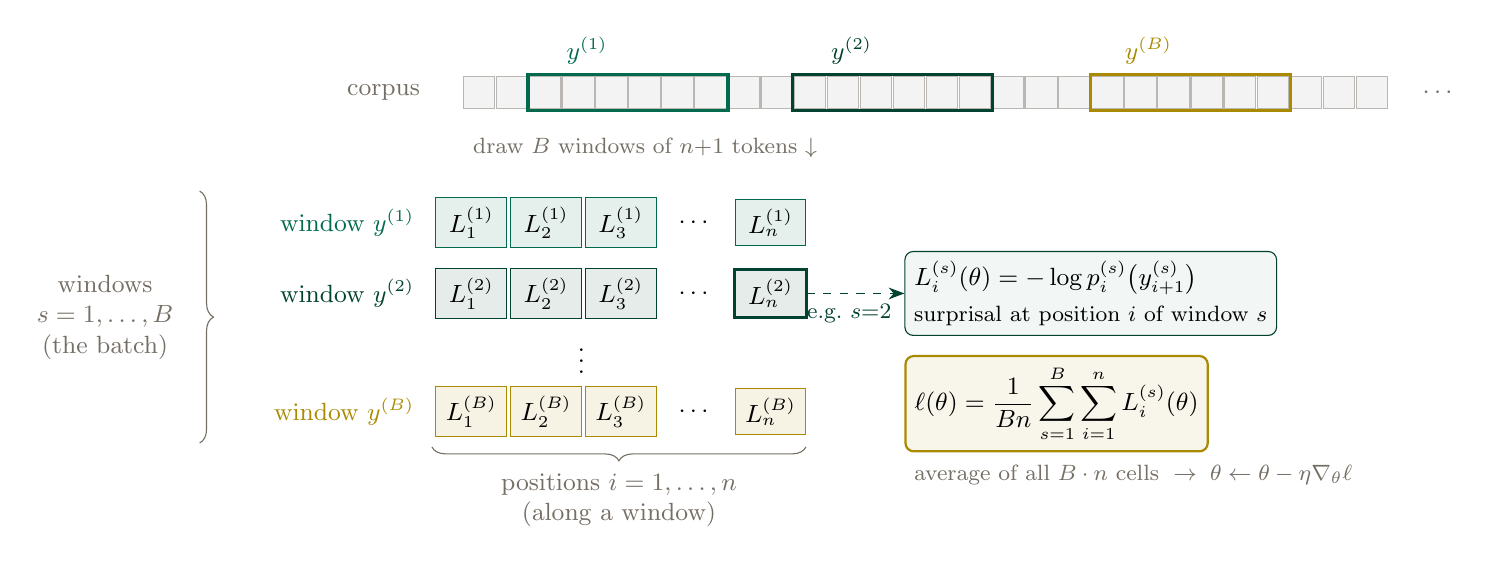
\begin{tikzpicture}[font=\small,>={Stealth[length=2mm]}]
% corpus strip
\node[anchor=west,text=gry] at (-0.2,2.55) {corpus};
\foreach \k in {0,...,27}{\draw[gry!50,fill=gry!8] ({0.42*\k+1.4},2.35) rectangle ({0.42*\k+1.8},2.75);}
\foreach \st/\col/\s in {2/acc/1,10/tea/2,19/gld/B}{
  \draw[\col,very thick] ({0.42*\st+1.38},2.32) rectangle ({0.42*(\st+5)+1.82},2.78);
}
\node[text=gry] at (13.8,2.55) {$\cdots$};
% batch rows
\def\cw{0.95}
\foreach \s/\lab/\col/\yy in {1/1/acc/0.9,2/2/tea/0,3/B/gld/-1.5}{
  \node[anchor=east,text=\col] at (0.9,\yy) {window $y^{(\lab)}$};
  \foreach \i in {1,2,3}{
    \node[draw=\col,fill=\col!10,minimum width=0.9cm,minimum height=0.55cm] (c\s\i) at ({1.5+\cw*(\i-1)},\yy) {$L^{(\lab)}_{\i}$};}
  \node at ({1.5+\cw*3},\yy) {$\cdots$};
  \node[draw=\col,fill=\col!10,minimum width=0.9cm,minimum height=0.55cm] (c\s n) at ({1.5+\cw*4},\yy) {$L^{(\lab)}_{n}$};
}
\node at (2.9,-0.75) {$\vdots$};
% labels on corpus windows
\node[text=acc,above] at (2.97,2.78) {$y^{(1)}$};
\node[text=tea,above] at (6.33,2.78) {$y^{(2)}$};
\node[text=gld,above] at (10.1,2.78) {$y^{(B)}$};
\node[text=gry,font=\footnotesize,anchor=west] at (1.4,1.85) {draw $B$ windows of $n{+}1$ tokens $\downarrow$};
% column braces
\draw[decorate,decoration={brace,mirror,amplitude=5pt},gry] (1.0,-1.95) -- node[below=6pt,align=center]{positions $i=1,\dots,n$\\(along a window)} (5.75,-1.95);
\draw[decorate,decoration={brace,amplitude=5pt},gry] (-1.95,1.3) -- node[left=6pt,align=center]{windows\\$s=1,\dots,B$\\(the batch)} (-1.95,-1.9);
% one cell detail
\node[draw=tea,rounded corners=3pt,fill=tea!5,align=left,anchor=west] (det) at (7.0,0.0)
 {$L_i^{(s)}(\theta)=-\log p_i^{(s)}\big(y^{(s)}_{i+1}\big)$\\[2pt]
  {\footnotesize surprisal at position $i$ of window $s$}};
\draw[tea,very thick] (c2n.south west) rectangle (c2n.north east);
\draw[->,tea,dashed] (c2n.east) -- (det.west);
\node[text=tea,font=\footnotesize] at (6.3,-0.25) {e.g.\ $s{=}2$};
% average
\node[draw=gld,thick,rounded corners=3pt,fill=gld!8,anchor=west] (avg) at (7.0,-1.4)
 {$\displaystyle \ell(\theta)=\frac{1}{Bn}\sum_{s=1}^{B}\sum_{i=1}^{n}L_i^{(s)}(\theta)$};
\node[anchor=west,text=gry,font=\footnotesize] at (7.0,-2.3) {average of all $B\cdot n$ cells $\;\to\;\theta\leftarrow\theta-\eta\nabla_\theta\ell$};
\end{tikzpicture}}
\end{center}
\end{frame}

\begin{frame}[t]{The derivative of the loss}
\begin{columns}[T]
\begin{column}{0.44\textwidth}
\begin{bxthm}
\small\textbf{Proposition} (predicted $-$ observed)\textbf{.}
\[
\frac{\partial L_i}{\partial z_i}=p_i-e_{y_{i+1}}\in\R^{|\Vc|}
\]
\end{bxthm}
{\small\textbf{Proof.} $\dfrac{\partial}{\partial z_{i,v}}\log\sum_u e^{z_{i,u}}=p_i(v)$ and $\dfrac{\partial z_{i,y_{i+1}}}{\partial z_{i,v}}=\one\{v=y_{i+1}\}$. $\blacksquare$\par}
\end{column}
\begin{column}{0.53\textwidth}
\begin{bxrem}
\small\textbf{Chain rule.}\footnotesize
\begin{align*}
\frac{\partial L_i}{\partial b}&=p_i-e_{y_{i+1}},\\
\frac{\partial L_i}{\partial \Wv}&=h_i\,(p_i-e_{y_{i+1}})^\top,\\
\frac{\partial L_i}{\partial h_i}&=\Wv\,(p_i-e_{y_{i+1}}),\\
\nabla_\theta\ell&=\frac1{Bn}\sum_{s,i}\frac{\partial L^{(s)}_i}{\partial z^{(s)}_i}\,\frac{\partial z^{(s)}_i}{\partial\theta}\\
&=\frac1{Bn}\sum_{s,i}\big(p^{(s)}_i-e_{y^{(s)}_{i+1}}\big)^{\!\top}\frac{\partial z^{(s)}_i}{\partial\theta}.
\end{align*}
\end{bxrem}
\end{column}
\end{columns}
\end{frame}

\begin{frame}[t]{Training: gradient descent on $\ell$}
\begin{columns}[T]
\begin{column}{0.5\textwidth}
\cfix
\begin{bxalg}
\small
\textbf{Input:} token corpus; $\theta_0$ random.\\
\uncover<2->{\textbf{for} $k=0,\dots,T-1$:}\\
\hspace*{1.2em}\uncover<3->{draw $y^{(1)},\dots,y^{(B)}\in\Vc^{\,n+1}$}\\
\hspace*{1.2em}\uncover<4->{forward pass: $\ell(\theta_k)$}\\
\hspace*{1.2em}\uncover<5->{backward pass: $\nabla_\theta\ell(\theta_k)$}\\
\hspace*{1.2em}\uncover<5->{$\theta_{k+1}=\theta_k-\eta\,\nabla_\theta\ell(\theta_k)$}\\
\uncover<6->{\textbf{return} $\theta_T$; freeze it.}\\[3pt]
{\color{gry}Toy run: $T=1000$, $B=8$, $n=16$.}
\end{bxalg}
\end{column}
\begin{column}{0.47\textwidth}
\cfix
\begin{bxdef}
\small\textbf{Trained:} $\theta=(E,P,\ \text{all } W_\bullet,b_\bullet,\gamma_\bullet,\beta_\bullet)$.\\
\textbf{Fixed:} $M,\sigma,d,h,L,n,\eta,T,B$.
\end{bxdef}
\begin{center}
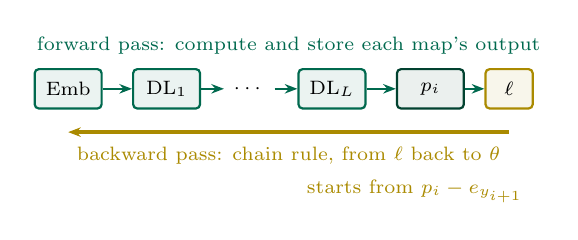
\begin{tikzpicture}[every node/.style={font=\scriptsize},>={Stealth[length=1.6mm]},
  st/.style={blk=acc,minimum width=0.85cm,minimum height=0.5cm}]
\node[st] (e) at (0,0) {$\Emb$}; \node[st] (d1) at (1.25,0) {$\DL_1$};
\node (dd) at (2.3,0) {$\cdots$}; \node[st] (dL) at (3.35,0) {$\DL_L$};
\node[blk=tea,minimum width=0.85cm,minimum height=0.5cm] (sm) at (4.6,0) {$p_i$};
\node[blk=gld,minimum width=0.6cm,minimum height=0.5cm] (l) at (5.6,0) {$\ell$};
\draw[->,acc,thick] (e)--(d1); \draw[->,acc,thick] (d1)--(dd); \draw[->,acc,thick] (dd)--(dL); \draw[->,acc,thick] (dL)--(sm); \draw[->,acc,thick] (sm)--(l);
\draw[->,gld,very thick] (5.6,-0.55) -- (0,-0.55);
\node[text=acc] at (2.8,0.55) {forward pass: compute and store each map's output};
\node[text=gld] at (2.8,-0.85) {backward pass: chain rule, from $\ell$ back to $\theta$};
\node[text=gld,anchor=east] at (5.9,-1.3) {starts from $p_i-e_{y_{i+1}}$};
\end{tikzpicture}
\end{center}
\end{column}
\end{columns}
\end{frame}

% ---------- Summary ---------------------------------------------------
\begin{frame}[t]{The whole map, and three take-aways}
\[
\small
\begin{CD}
\Vc^{\,n} @>{\Emb}>> \R^{n\times d} @>{\DL_L\circ\cdots\circ\DL_1}>> \R^{n\times d} @>{\LN_f,\ \Wv,\ b}>> \R^{n\times|\Vc|} @>{\softmax_{\rm row}}>> \Delta(\Vc)^n
\end{CD}
\]
\[
\DL_l=\FFNB_l\circ\AttnB_l,\qquad l=1,\dots,L.
\]
\begin{columns}[T]
\begin{column}{0.32\textwidth}
\cfix
\begin{bxthm}
\small\textbf{1. Objective.} $\min_\theta\ell(\theta)$,\ \ $\partial L_i/\partial z_i=p_i-e_{y_{i+1}}$.
\end{bxthm}
\end{column}
\begin{column}{0.32\textwidth}
\cfix
\begin{bxdef}
\small\textbf{2. Architecture.} $\DL=\FFNB\circ\AttnB$; skips $\oplus$ and $\LN$.
\end{bxdef}
\end{column}
\begin{column}{0.32\textwidth}
\cfix
\begin{bxrem}
\small\textbf{3. Mask.} $p_i=\pi_\theta(\,\cdot\mid y_{\le i})$.
\end{bxrem}
\end{column}
\end{columns}
\vspace{0.5em}
\begin{center}
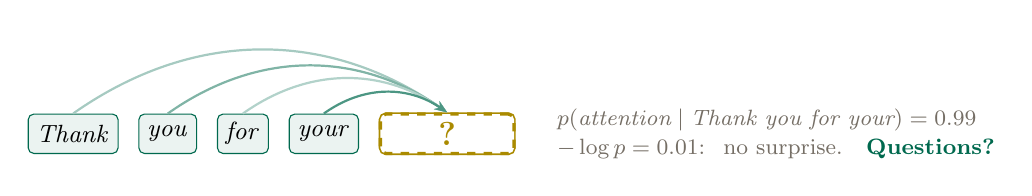
\begin{tikzpicture}[visible on=<2->,every node/.style={font=\small},>={Stealth[length=1.6mm]},
  tk/.style={draw=acc,rounded corners=2pt,fill=acc!8,inner sep=3pt,minimum height=0.5cm}]
\node[tk] (t1) at (0,0) {\textit{Thank}};
\node[tk,right=0.25cm of t1] (t2) {\textit{you}};
\node[tk,right=0.25cm of t2] (t3) {\textit{for}};
\node[tk,right=0.25cm of t3] (t4) {\textit{your}};
\node[draw=gld,very thick,rounded corners=2pt,fill=gld!15,inner sep=3pt,minimum height=0.5cm,right=0.25cm of t4,font=\small\bfseries] (t5) {attention};
\node[draw=gld,very thick,dashed,rounded corners=2pt,fill=white,inner sep=3pt,minimum height=0.5cm,font=\small\bfseries,visible on=<2>] at (t5) {\phantom{attention}};
\node[text=gld,font=\large\bfseries,visible on=<2>] at (t5) {?};
\foreach \j/\op in {1/35,2/50,3/30,4/70}{\draw[->,acc!\op,thick,visible on=<3->] (t\j.north) to[bend left=35] (t5.north);}
\node[anchor=west,text=gry,font=\footnotesize,align=left,visible on=<3->] at ([xshift=0.4cm]t5.east)
 {$p(\textit{attention}\mid\textit{Thank you for your})=0.99$\\[1pt]
  $-\log p=0.01$: \ no surprise.\quad \textbf{\color{acc}Questions?}};
\end{tikzpicture}
\end{center}
\end{frame}

% ---------- References ------------------------------------------------
\section{References}
\begin{frame}[t]{References}
\small
\begin{itemize}\setlength{\itemsep}{4pt}
\item Shannon, C.\,E. (1948). A mathematical theory of communication. \emph{Bell System Technical Journal} 27. \ (See also Shannon 1951, Prediction and entropy of printed English.)
\item Rosenblatt, F. (1958). The perceptron: a probabilistic model for information storage and organization in the brain. \emph{Psychological Review} 65.
\item Vaswani, A., et al.\ (2017). Attention is all you need. \emph{NeurIPS}.
\item Radford, A., Narasimhan, K., Salimans, T., \& Sutskever, I. (2018). Improving language understanding by generative pre-training. OpenAI.
\end{itemize}
\end{frame}

\end{document}
